%Copyright 2019 Christopher M. Jermaine (cmj4@rice.edu) and Risa B. Myers (rbm2@rice.edu)
%
%Licensed under the Apache License, Version 2.0 (the "License");
%you may not use this file except in compliance with the License.
%You may obtain a copy of the License at
%
%    https://www.apache.org/licenses/LICENSE-2.0
%
%Unless required by applicable law or agreed to in writing, software
%distributed under the License is distributed on an "AS IS" BASIS,
%WITHOUT WARRANTIES OR CONDITIONS OF ANY KIND, either express or implied.
%See the License for the specific language governing permissions and
%limitations under the License.
%===============================================================
\documentclass[aspectratio=169]{beamer}
\mode<presentation> 
{
\usetheme[noshadow, minimal,numbers,riceb,nonav]{Rice}
\usefonttheme[onlymath]{serif}
\setbeamercovered{transparent}
}
\useinnertheme{rectangles}
\usepackage{multirow}

\usepackage[english]{babel}

 \usepackage{color}
 \usepackage{mathptmx}
\usepackage{helvet}
\usepackage{courier}
\usepackage[T1]{fontenc}
\usepackage{trajan}
\usepackage{ textcomp }
\usepackage{listings}

\newenvironment{noindentitemize}
{ \begin{itemize}
 \setlength{\itemsep}{1.5ex}
  \setlength{\parsep}{0pt}   
  \setlength{\parskip}{0pt}
 \addtolength{\leftskip}{-2em}
 }
{ \end{itemize} }

\newenvironment{noindentitemize2}
{ \begin{itemize}
  \setlength{\itemsep}{0ex}
  \setlength{\parskip}{0pt}
  \setlength{\parsep}{0pt}   
  \addtolength{\leftskip}{-2em}  }
{ \end{itemize} }



\lstnewenvironment{SQL}
  {\lstset{
        aboveskip=5pt,
        belowskip=5pt,
        escapechar=!,
        mathescape=true,
        upquote=true,
        language=SQL,
        basicstyle=\linespread{0.94}\ttfamily\footnotesize,
        morekeywords={PRINT, CURSOR, OPEN, FETCH, CLOSE, DECLARE, BEGIN, END, PROCEDURE, FOR, EACH, WITH, PARTITION, 	TEST, WHETHER, PROBABILITY, OUT,LOOP,IF,CONTINUE, HANDLER,CALL, FUNCTION, RETURNS, LANGUAGE,BODY,RETURN, REPLACE,plpgsql,
        RAISE, NOTICE,
        REPLACE, ROW, BEFORE, EXIT, TEXT, REFCURSOR, QUOTE_LITERAL, DELIMITER,CONCAT,FOUND,LEAVE },
        deletekeywords={VALUE, PRIOR},
        showstringspaces=true}
        \vspace{0pt}
        \noindent\minipage{0.65\textwidth}}
  {\endminipage\vspace{0pt}}
  
  
\lstnewenvironment{SQLtiny}
  {\lstset{
        aboveskip=5pt,
        belowskip=5pt,
        escapechar=!,
        mathescape=true,
        upquote=true,
        language=SQL,
        basicstyle=\linespread{0.94}\ttfamily\tiny,
        morekeywords={PRINT, CURSOR, OPEN, FETCH, CLOSE, DECLARE, BEGIN, END, PROCEDURE, FOR, EACH, WITH, PARTITION, 	TEST, WHETHER, PROBABILITY, OUT,LOOP,IF,CONTINUE, HANDLER,CALL, FUNCTION, RETURNS, LANGUAGE,BODY,RETURN, REPLACE,plpgsql,
        RAISE, NOTICE,
        REPLACE, ROW, BEFORE, EXIT, TEXT, REFCURSOR, QUOTE_LITERAL, DELIMITER,CONCAT,FOUND,LEAVE },
       deletekeywords={VALUE, PRIOR},
        showstringspaces=true}
        \vspace{0pt}%
        \noindent\minipage{0.47\textwidth}}
  {\endminipage\vspace{0pt}}

%===============================================================%

\title[]
{Tools \& Models for Data Science}

\subtitle{Intro to Supervised Learning}

\author[]{Chris Jermaine \& Risa Myers}
\institute
{
  Rice University 
}

\date[]{}

\subject{Beamer}


\begin{document}

\begin{frame}
 \titlepage
\end{frame}

%***********************************************************
\begin{frame}{Machine Learning (Review)}

\begin{itemize}
\item Predicting / classifying new data based on what we have learned from existing data
\item Requires the training data to be representative of the data we want to predict / classify
\item Tasks
	\begin{itemize}
	\item 1. Choosing the model---choose family, complexity, hyperparameters
	\item 2. Learning the model---``fit'' model to data by adjusting parameters
	\item 3. Validating the model---make sure model matches data
	\item 4. Applying the model---use the model to explain past/present make predictions on future
	\end{itemize}
\end{itemize}
\end{frame}
%***********************************************************
\begin{frame}{``Supervised'' Learning}

\begin{itemize}
\item One of the most fundamental problems in data science
	\begin{itemize}
	\item Given a bunch of $(x_i, y_i)$ pairs
	\item Where $x_i$ is a feature vector for data $i$
	\item And $y_i$ is the label for $x_i$ 
	\item Goal: learn how to predict value of $y$ from $x$
	\item Called ``supervised'' because have examples of correct labeling
	\end{itemize}
\end{itemize}
\end{frame}
%***********************************************************
\begin{frame}{Problem Examples}

\begin{itemize}
\item From research done at Rice:
\begin{itemize}
                \item Given a text clinical note, label ``breast cancer'' or not
                \item Given a document (email) in a court case, figure which subjects pertain % eDiscovery  ``Sift'' through millions of emails to determine the topics and find the small set that are relevant to a legal case
                \item Given information about a patient surgery, predict death
		\item Given head trauma patient info, predict intracranial pressure crisis
		\item Given an set of surgical vital signs, label ``good surgery'' or not % because this correlates with outcomes
		\item Predict location and damage from a hurricane
		\item Many others!
\end{itemize}
\end{itemize}
\end{frame}
%***********************************************************
\begin{frame}{Two Most Common Examples of Supervised Learning}

\begin{itemize}
\item Classification and regression
\item Classification:
	\begin{itemize}
	\item Outcome to predict is in $\{+1, -1\}$ (``yes'' or ``no''), (``True'' or ``False'')
	\item Ex: Given a text clinical note, label it as ``breast cancer'' or not
	\end{itemize}
\item Regression:
	\begin{itemize}
	\item Outcome to predict is a real number
	\item Ex: Given an ad, predict number of clickthrus per hour
	\end{itemize}
\end{itemize}
\end{frame}
%***********************************************************
\begin{frame}{What Models Are Used?}

\begin{itemize}
\item Many!
	\begin{itemize}
	\item We will cover a number of them
	\item Simplest, most common: linear regression.  From $x_i$, predict $y_i$ as:
	$$ \sum_j x_{i,j} r_j$$
	\item Where $x_{i,j}$ is a matrix of rows of feature values, one for each data point
	\item $\langle r_1, r_2, ..., r_m \rangle$ are called regression coefficients
		\begin{itemize}
		\item The relative magnitude of the regression coefficient tells you how important each feature is
		\end{itemize}
	\item Other common ones: kNN, support vector machines
	\end{itemize}
\end{itemize}
\end{frame}
%***********************************************************
\begin{frame}{What do we Mean by Features?}

%\begin{columns}
%\begin{column}{0.2\textwidth}
\begin{itemize}
\item Music
	\begin{itemize}
	\item Artist name
	\item Song duration
	\item Key
	\item Loudness
	\item Tempo
	\item Year
	\item $\ldots$
	\end{itemize}
%\item Patient
%	\begin{itemize}
%	\item Age
%	\item History of Smoking
%	\item History of Diabetes
%	\item Blood pressure
%	\item Weight
%	\item $\ldots$
%	\end{itemize}
\end{itemize}
%\end{column}
%\begin{column}{0.8\textwidth}
{\tiny
\begin {table}[H]
\begin{tabular}{|r|r|r|r|r|r|r|}
\hline
& 	artist &  &   &  &  &   \\ 
 songId & name &  duration & key &  loudness & tempo & year   \\ \hline \hline
SONHOTT12A8C13493C  & Adam Ant & 233 & 0  & -9.013 & 119.293 & 1982 \\ \hline
SOGNQWU12A8AE4868F  & Eurythmics & 207 & 0  & -6.629 & 84.164 & 1985 \\ \hline
SOZWHVZ12A6D4F90E7  & U2 & 485 & 3  & -7.614 & 134.083 & 2007 \\ \hline
SOGOQGE12AB0182907  & The Killers & 284 & 4  & -6.546	 & 151.953 & 2008 \\ \hline
SONCHNB12AB01849A2  & Wade Ray & 136  & 3  & -9.713	 & 171.527& 2005 \\ \hline

\end{tabular}
\end{table}
}
%\end{column}
%\end{columns}
\end{frame}
%***********************************************************
\begin{frame}{Labels}

%\begin{columns}
%\begin{column}{0.4\textwidth}
\begin{itemize}
\item Some outcome / value / output pertaining to the data
\end{itemize}
%\end{column}
%\begin{column}{0.6\textwidth}
{\tiny
\begin {table}[H]
\begin{tabular}{|r|r||r|r|r|r|r|r|r|r|}
\hline
 & & 	& artist &  &   &  &  &   \\ 
Familiarity & Familiarity $\ge$ 0.8 & songId & name &  duration & key &  loudness & tempo & year   \\ \hline \hline
0.63 & FALSE & SONHOTT12A8C13493C  & Adam Ant & 233 & 0  & -9.013 & 119.293 & 1982 \\ \hline
0.75 & FALSE & SOGNQWU12A8AE4868F  & Eurythmics & 207 & 0  & -6.629 & 84.164 & 1985 \\ \hline
0.84 & TRUE & SOZWHVZ12A6D4F90E7  & U2 & 485 & 3  & -7.614 & 134.083 & 2007 \\ \hline
0.92 & TRUE & SOGOQGE12AB0182907  & The Killers & 284 & 4  & -6.546	 & 151.953 & 2008 \\ \hline
0.05 & FALSE & SONCHNB12AB01849A2  & Wade Ray & 136  & 3  & -9.713	 & 171.527& 2005 \\ \hline

\end{tabular}
\end{table}
}
%\end{column}
%\end{columns}
\end{frame}
%***********************************************************
\begin{frame}{A Model to Predict Music Familiarity: Regression Coeffiecients}

\begin{columns}
\begin{column}{0.4\textwidth}
	$$ \sum_j x_{i,j} r_j$$
\begin{enumerate}
\item Learn the regression coefficients
\item Use the model
\begin{enumerate}
\item Plug in the value of each feature for each song 
\item Get a real valued output
\item Apply a function to convert it to a binary classification
\end{enumerate}
\end{enumerate}
\end{column}
\begin{column}{0.6\textwidth}
{\tiny
\begin {table}[H]
\begin{tabular}{|r|r|}
\hline
Feature & Regression Coefficient \\ \hline
artist.hotttnesss      &      -25.5347\\ \hline
artist.mbtags\_count   &          -0.18\\ \hline
bars\_confidence    &           -0.3755\\ \hline
bars\_start              &       0.0893\\ \hline
beats\_confidence   &             0.407\\ \hline
beats\_start          &          0.1196\\ \hline
duration              &         0.0047\\ \hline
end\_of\_fade\_in      &           0.0261\\ \hline
key                     &      -0.0076\\ \hline
key\_confidence     &            0.3139\\ \hline
latitude               &        0.0022\\ \hline
longitude          &            0.0019\\ \hline
loudness         &             -0.1131\\ \hline
mode                 &         -0.0399\\ \hline
mode\_confidence &               0.3354\\ \hline
release.id                &          0\\ \hline
song\_hotttnesss      &         -1.6807\\ \hline
start\_of\_fade\_out     &        -0.0043\\ \hline
tatums\_confidence      &        0.7883\\ \hline
tatums\_start              &    -0.2762\\ \hline
tempo                        &  0.0015\\ \hline
terms\_freq               &      0.0006\\ \hline
time\_signature           &     -0.0579\\ \hline
time\_signature\_confidence  &    -0.203\\ \hline
year                         &  0.0001\\ \hline
Intercept                   &  13.7194\\ \hline
\end{tabular}
\end{table}
}
\end{column}
\end{columns}
\end{frame}

%***********************************************************
\begin{frame}{Measuring Classification Accuracy: TP, FP, FN, TN}

\begin{itemize}
\item True Positive (TP) -- model predicts TRUE when label is TRUE
\item False Positive (FP) -- model predicts TRUE when label is FALSE
\item True Negative (TN) -- model predicts FALSE when label is FALSE
\item False Negative (FN) -- model predicts FALSE when label is TRUE
\end{itemize}

\end{frame}
%***********************************************************
\begin{frame}{Measuring Classification Accuracy: Confusion Matrix}

\begin{itemize}
\item Tabular representation of results 
\end{itemize}
\begin{tabular}{|c|c|r|r|r|} \hline
\multicolumn{2}{|c|}{}   &   \multicolumn{2}{c|}{Predicted}  & \\ \cline{3-4}
\multicolumn{2}{|c|}{} & Negative & Positive  & \\ \hline  
\multirow{2}{*}{Actual} & Negative & TN & FP  & Total Negative \\ \cline{2-5}
 & Positive & FN & TP  & Total Positive \\ \hline \hline
 \multicolumn{2}{|c|}{} &  Total Predicted & Total Predicted &  \\ 
 \multicolumn{2}{|c|}{Total} &  Negative&  Positive & \\ \hline
 \end{tabular}

\end{frame}
%***********************************************************
\begin{frame}{Measuring Classification Accuracy: Confusion Matrix}

\begin{itemize}
\item Tabular representation of results 
\end{itemize}
\begin{tabular}{|c|c|r|r|r|} \hline
\multicolumn{2}{|c|}{}   &   \multicolumn{2}{c|}{Predicted}  & \\ \cline{3-4}
\multicolumn{2}{|c|}{} & Negative & Positive  & \\ \hline  
\multirow{2}{*}{Actual} & Negative & 8954 & 178  & 9132 \\ \cline{2-5}
 & Positive & 335 & 533  & 868 \\ \hline \hline
 \multicolumn{2}{|c|}{Total} & 9289 & 711  & 10000\\ \hline
 \end{tabular}

\end{frame}
%***********************************************************
\begin{frame}{Measuring Classification Accuracy: \% Correct}

\begin{itemize}
\item Simplest: \% correct
\item $\frac{\textrm{TP + TN}}{\textrm{P + N}} = \frac{533+8954}{868 + 9132} = 0.95$

	\item[?] Pros and cons?
\end{itemize}

\begin{tabular}{|c|c|r|r|r|} \hline
\multicolumn{2}{|c|}{}   &   \multicolumn{2}{c|}{Predicted}  & \\ \cline{3-4}
\multicolumn{2}{|c|}{} & Negative & Positive  & \\ \hline  
\multirow{2}{*}{Actual} & Negative & 8954 & 178  & 9132 \\ \cline{2-5}
 & Positive & 335 & 533  & 868 \\ \hline \hline
 \multicolumn{2}{|c|}{Total} & 9289 & 711  & 10000\\ \hline
 \end{tabular}

\end{frame}
%***********************************************************
\begin{frame}{Measuring Classification Accuracy: \% Correct}

\begin{itemize}
\item Simplest: \% correct
	\begin{itemize}
	\item Pros
		\begin{itemize}
		\item Easy to interpret
		\item Easy to compute
		\item Easy to compare
		\end{itemize}
	\item Cons
		\begin{itemize}
		\item Certain classes may be more important than others
		\item E.g. Male breast cancer
		\item Can achieve high accuracy just by saying ``No''
		\item In this case, better to find all the cases and some that aren't
		\end{itemize}
	\end{itemize}
\end{itemize}
\end{frame}
%***********************************************************
\begin{frame}{Measuring Classification Accuracy: FP \& FN}

\begin{columns}
\begin{column}{0.5\textwidth}
{\tiny
\begin{tabular}{|c|c|r|r|r|} \hline
\multicolumn{2}{|c|}{}   &   \multicolumn{2}{c|}{Predicted}  & \\ \cline{3-4}
\multicolumn{2}{|c|}{} & Negative & Positive  & \\ \hline  
\multirow{2}{*}{Actual} & Negative & TN & FP  & Total Negative \\ \cline{2-5}
 & Positive & FN & TP  & Total Positive \\ \hline \hline
 \multicolumn{2}{|c|}{} &  Total Predicted & Total Predicted &  \\ 
 \multicolumn{2}{|c|}{Total} &  Negative&  Positive & \\ \hline
 \end{tabular}
 }
 \end{column}
\begin{column}{0.5\textwidth}
{\tiny
\begin{tabular}{|c|c|r|r|r|} \hline
\multicolumn{2}{|c|}{}   &   \multicolumn{2}{c|}{Predicted}  & \\ \cline{3-4}
\multicolumn{2}{|c|}{} & Negative & Positive  & \\ \hline  
\multirow{2}{*}{Actual} & Negative & 8954 & 178  & 9132 \\ \cline{2-5}
 & Positive & 335 & 533  & 868 \\ \hline \hline
 \multicolumn{2}{|c|}{Total} & 9289 & 711  & 10000\\ \hline
 \end{tabular}
 }
 \end{column}
 \end{columns}
\small{
	\begin{itemize}
	\item False positive: \% of those we say are ``yes'' that are not really ``yes''
	$$\frac{FP}{N} = \frac{FP}{FP + TN} = \frac{178}{8954 + 178} = 0.19$$
	\item False negative: \% of those we say are ``no'' that are not really ``no''
	$$\frac{FN}{P} = \frac{FN}{FN + TP} = \frac{335}{335 + 533} = 0.39$$
	\item Simple concept, easy to get wrong
	\item Male breast cancer: 50\% FP rate is okay: 3 real cases + 3 extra cases
	\item Alert fatigue: 72 - 99\%  of alerts are not actual causes for alert  \footnote{Sendelbach S, Funk M. Alarm fatigue: a patient safety concern. AACN advanced critical care. 2013;24(4):378-86.}
	\end{itemize}
	}
\end{frame}
%***********************************************************
\begin{frame}{Measuring Classification Accuracy: Recall \& Precision}
\begin{columns}
\begin{column}{0.7\textwidth}
\begin{itemize}
	\item Recall (Sensitivity): \% of those that are really ``yes'' that we say are ``yes''
	$$\frac{TP}{P} = \frac{TP}{TP + FN} = \frac{533}{533 + 335} = 0.61$$
	\item Precision: \% of those that we say are ``yes'' that are really ``yes''
	$$\frac{TP}{TP + FP} = \frac{533}{533 + 178} = 0.75 $$
\end{itemize}
\tiny{Image credit:
\url{https://en.wikipedia.org/wiki/Precision_and_recall\#/media/File:Precisionrecall.svg}
}
\end{column}
\begin{column}{0.3\textwidth}
    \includegraphics[width=1\textwidth]{lectSup/precisionrecall} \tiny{\footnote{\url{www.}}}

\end{column}
\end{columns}

\end{frame}
%***********************************************************
\begin{frame}{Measuring Classification Accuracy: Recall \& Precision}

\begin{columns}[c]
\begin{column}{0.7\textwidth}

\begin{tabular}{|c|c|r|r|r|} \hline
\multicolumn{2}{|c|}{}   &   \multicolumn{2}{c|}{Predicted}  & \\ \cline{3-4}
\multicolumn{2}{|c|}{} & Negative & Positive  & \\ \hline  
\multirow{2}{*}{Actual} & Negative & 0 & 9132  & 9132 \\ \cline{2-5}
 & Positive & 0 & 868  & 868 \\ \hline \hline
 \multicolumn{2}{|c|}{Total} & 0 & 868  & 10000\\ \hline
 \end{tabular}
\end{column}
\begin{column}{0.3\textwidth}

\begin{tabular}{|c|c|c|c|} \hline
TN & FP\\ \hline
FN & TP \\ \hline
 \end{tabular}
\end{column}
\end{columns}
\begin{itemize}
	\item[?] What is our Recall if we call all of the data points Positive?
	$$\frac{TP}{TP + FN} = $$
\end{itemize}

	
\end{frame}
%***********************************************************
\begin{frame}{Measuring Classification Accuracy: Recall \& Precision}

\begin{columns}[c]
\begin{column}{0.7\textwidth}

\begin{tabular}{|c|c|r|r|r|} \hline
\multicolumn{2}{|c|}{}   &   \multicolumn{2}{c|}{Predicted}  & \\ \cline{3-4}
\multicolumn{2}{|c|}{} & Negative & Positive  & \\ \hline  
\multirow{2}{*}{Actual} & Negative & 0 & 9132  & 9132 \\ \cline{2-5}
 & Positive & 0 & 868  & 868 \\ \hline \hline
 \multicolumn{2}{|c|}{Total} & 0 & 868  & 10000\\ \hline
 \end{tabular}
\end{column}
\begin{column}{0.3\textwidth}

\begin{tabular}{|c|c|c|c|} \hline
TN & FP\\ \hline
FN & TP \\ \hline
 \end{tabular}
\end{column}
\end{columns}
\begin{itemize}
	\item What is our Recall if we call all of the data points Positive?
	$$\frac{TP}{TP + FN} = \frac{868}{868+0} = 1$$
	\item[?] What is our Precision if we call all of the data points Positive?
	$$\frac{TP}{TP+FP} = $$
\end{itemize}

	
\end{frame}
%***********************************************************
\begin{frame}{Measuring Classification Accuracy: Recall \& Precision}

\begin{columns}[c]
\begin{column}{0.7\textwidth}

\begin{tabular}{|c|c|r|r|r|} \hline
\multicolumn{2}{|c|}{}   &   \multicolumn{2}{c|}{Predicted}  & \\ \cline{3-4}
\multicolumn{2}{|c|}{} & Negative & Positive  & \\ \hline  
\multirow{2}{*}{Actual} & Negative & 0 & 9132  & 9132 \\ \cline{2-5}
 & Positive & 0 & 868  & 868 \\ \hline \hline
 \multicolumn{2}{|c|}{Total} & 0 & 868  & 10000\\ \hline
 \end{tabular}
\end{column}
\begin{column}{0.3\textwidth}

\begin{tabular}{|c|c|c|c|} \hline
TN & FP\\ \hline
FN & TP \\ \hline
 \end{tabular}
\end{column}
\end{columns}
\begin{itemize}
	\item What is our Recall if we call all of the data points Positive?
	$$\frac{TP}{TP + FN} = \frac{868}{868+0} = 1$$
	\item What is our Precision if we call all of the data points Positive?
	$$\frac{TP}{TP+FP} = \frac{868}{868 + 9132} = 0.09$$
\end{itemize}

	
\end{frame}

%
%%***********************************************************
%\begin{frame}{Measuring Classification Accuracy: Recall \& Precision}
%\begin{columns}
%\begin{column}{0.5\textwidth}
%{\tiny
%\begin{tabular}{|c|c|r|r|r|} \hline
%\multicolumn{2}{|c|}{}   &   \multicolumn{2}{c|}{Predicted}  & \\ \cline{3-4}
%\multicolumn{2}{|c|}{} & Negative & Positive  & \\ \hline  
%\multirow{2}{*}{Actual} & Negative & TN & FP  & Total Negative \\ \cline{2-5}
% & Positive & FN & TP  & Total Positive \\ \hline \hline
% \multicolumn{2}{|c|}{} &  Total Predicted & Total Predicted &  \\ 
% \multicolumn{2}{|c|}{Total} &  Negative&  Positive & \\ \hline
% \end{tabular}
% }
% \end{column}
%\begin{column}{0.5\textwidth}
%{\tiny
%\begin{tabular}{|c|c|r|r|r|} \hline
%\multicolumn{2}{|c|}{}   &   \multicolumn{2}{c|}{Predicted}  & \\ \cline{3-4}
%\multicolumn{2}{|c|}{} & Negative & Positive  & \\ \hline  
%\multirow{2}{*}{Actual} & Negative & 8954 & 178  & 9132 \\ \cline{2-5}
% & Positive & 335 & 533  & 868 \\ \hline \hline
% \multicolumn{2}{|c|}{Total} & 9289 & 711  & 10000\\ \hline
% \end{tabular}
% }
% \end{column}
% \end{columns}
%
%\begin{itemize}
%	\item Recall (Sensitivity): \% of those that are really ``yes'' that we say are ``yes''
%	$$\frac{TP}{P} = \frac{TP}{TP + FN} = \frac{10}{10 + 2}$$
%	\item Precision: \% of those that we say are ``yes'' that are really ``yes''
%	$$\frac{TP}{TP + FP} = \frac{10}{10 + 5}$$
%	\item[?] Pros and cons?
%\end{itemize}
%\end{frame}
%***********************************************************
\begin{frame}{Measuring Classification Accuracy: Recall \& Precision}

\begin{itemize}
\item Recall and precision
	\begin{itemize}
	\item Pros
		\begin{itemize}
		\item More information than accuracy
		\item Tolerance for TP and FN can be different, based on the situation
		\end{itemize}
	\item Cons
		\begin{itemize}
		\item Can be confusing
		\item There are two numbers (Precision and Recall) to compare
		\end{itemize}
	\end{itemize}
\end{itemize}
\end{frame}
%***********************************************************
\begin{frame}{Measuring Classification Accuracy $F1$-score}

\begin{itemize}
\item $F_1$
	\begin{itemize}
	\item Puts recall and precision into single number
	$$F_1 = \frac{2 \times \textrm{ precision } \times \textrm{ recall }}{\textrm{ precision } + \textrm{ recall }}$$
	\item Ranges from 0 to 1
	\item 1 is best
	\item Also called the harmonic average of precision and recall
	\end{itemize}
\end{itemize}
\end{frame}
%***********************************************************
\begin{frame}{Digression: Mean Blood Pressure}

\begin{itemize}
\item Blood Pressure has two components: Systolic and Diastolic
\item Systolic -- 1st number; pressure when heart is beating
\item Diastolic -- 2nd number; pressure when heart is resting
\item Mean BP is NOT 
$$ \frac{\textrm{Systolic} + \textrm{Diastolic}}{2}$$
\item Instead it is 
$$ \frac{\textrm{Systolic} + 2 * \textrm{Diastolic}}{3}$$

\end{itemize}
\end{frame}
%***********************************************************
\begin{frame}{Measuring Classification Accuracy: F-scores}

\begin{itemize}
\item $F_1$
	$$F_1 = \frac{2 \times \textrm{ precision } \times \textrm{ recall }}{\textrm{ precision } + \textrm{ recall }}$$
\item Pros
		\begin{itemize}
		\item Reasonable way to combine precision and recall	
		\end{itemize}
\item Cons
		\begin{itemize}
		\item Somewhat arbitrary
		\item Could use F$_2$, F$_3$, etc.
	$$F_\beta = (1 + \beta^2) \times \frac{\textrm{ precision } \times \textrm{ recall }}{(\beta^2\times\textrm{ precision }) + \textrm{ recall }}$$
		\end{itemize}
\end{itemize}
\end{frame}

%***********************************************************
\begin{frame}{Measuring Classification Accuracy: $F$-scores on Our Model}

\begin{itemize}
\item 	$F_1 = 0.68$
\item 	$F_2 = 0.64$
\item 	$F_3 = 0.63$
	
\end{itemize}
\end{frame}


%***********************************************************
\begin{frame}{AUC ROC}

\begin{columns}
\begin{column}{0.5\textwidth}
    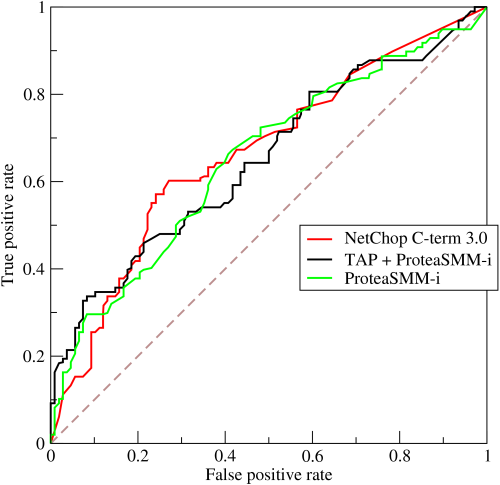
\includegraphics[width=1\textwidth]{lectSup/Roccurves}
   
   \vspace{-1em}
    {\tiny Image credit: \url{https://commons.wikimedia.org/
    wiki/File:Roccurves.png}}
\end{column}
\begin{column}{0.5\textwidth}

\begin{itemize}
	\item ROC = ``Receiver operating characteristic'' 
	\item AUC = ``Area under curve''
	\item Measure of how well the classes are separated
	\item Use for ``tunable'' classifiers (with cut-offs, like Logistic Regression)
	\item Gives single number $\le$ 1.0
	\item Less than 0.5 means ``actively bad''
	\item[?] Often shown with the diagonal. Why?
	\item[?] What does it mean if you have an AUC < 0.5? % classes are flipped, or some other error
\end{itemize}
\end{column}
\end{columns}
\end{frame}
%***********************************************************
\begin{frame}{Measuring Classification Accuracy: $F$-scores on Our Model}

    \includegraphics[width=1\textwidth]{/Users/rbm2/Desktop/roc.jpeg}
\end{frame}
%***********************************************************
\begin{frame}{AUC ROC: Pros and Cons}

\begin{columns}
\begin{column}{0.5\textwidth}
    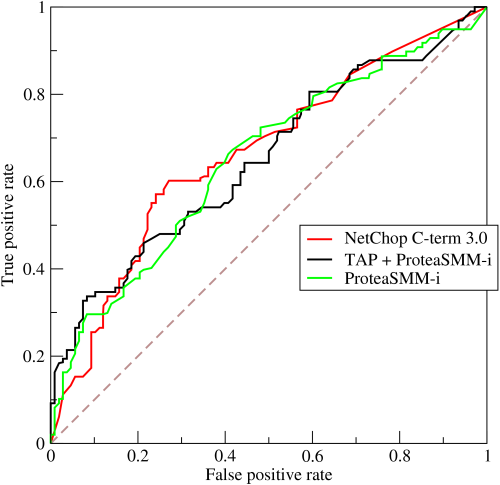
\includegraphics[width=1\textwidth]{lectSup/Roccurves} %https://commons.wikimedia.org/wiki/File:Roccurves.png

   
   \vspace{-1em}
    {\tiny Image credit: \url{https://commons.wikimedia.org/
    wiki/File:Roccurves.png}}

\end{column}
\begin{column}{0.5\textwidth}

\begin{itemize}
	\item Pros
		\begin{itemize}
		\item Single number
		\item Well known
		\item Immune to classification threshold
		\end{itemize}
	\item Cons
		\begin{itemize}
		\item Only works on binary classification
		\end{itemize}
	\end{itemize}
\end{column}
\end{columns}
\end{frame}
%***********************************************************
\begin{frame}{AUC ROC: Intuition}

\begin{columns}
\begin{column}{0.5\textwidth}
    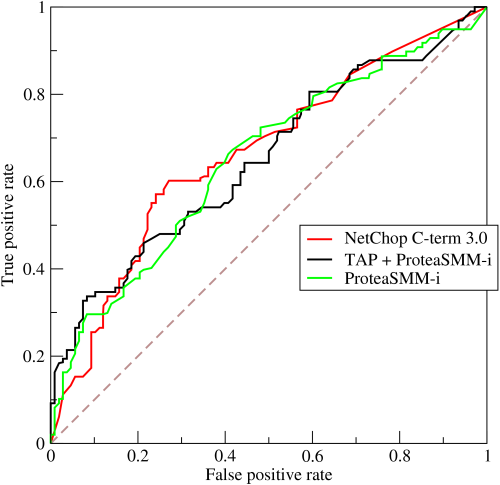
\includegraphics[width=1\textwidth]{lectSup/Roccurves} %https://commons.wikimedia.org/wiki/File:Roccurves.png

   
   \vspace{-1em}
    {\tiny Image credit: \url{https://commons.wikimedia.org/
    wiki/File:Roccurves.png}}

\end{column}
\begin{column}{0.5\textwidth}

\begin{itemize}
	\item Requires us to have a numeric value for the results that are mapped to a binary value
	\item Depending on where we set the threshold, we get different results
\end{itemize}
\end{column}
\end{columns}
\end{frame}

%***********************************************************
\begin{frame}{AUC ROC}

\begin{columns}
\begin{column}{0.2\textwidth}
    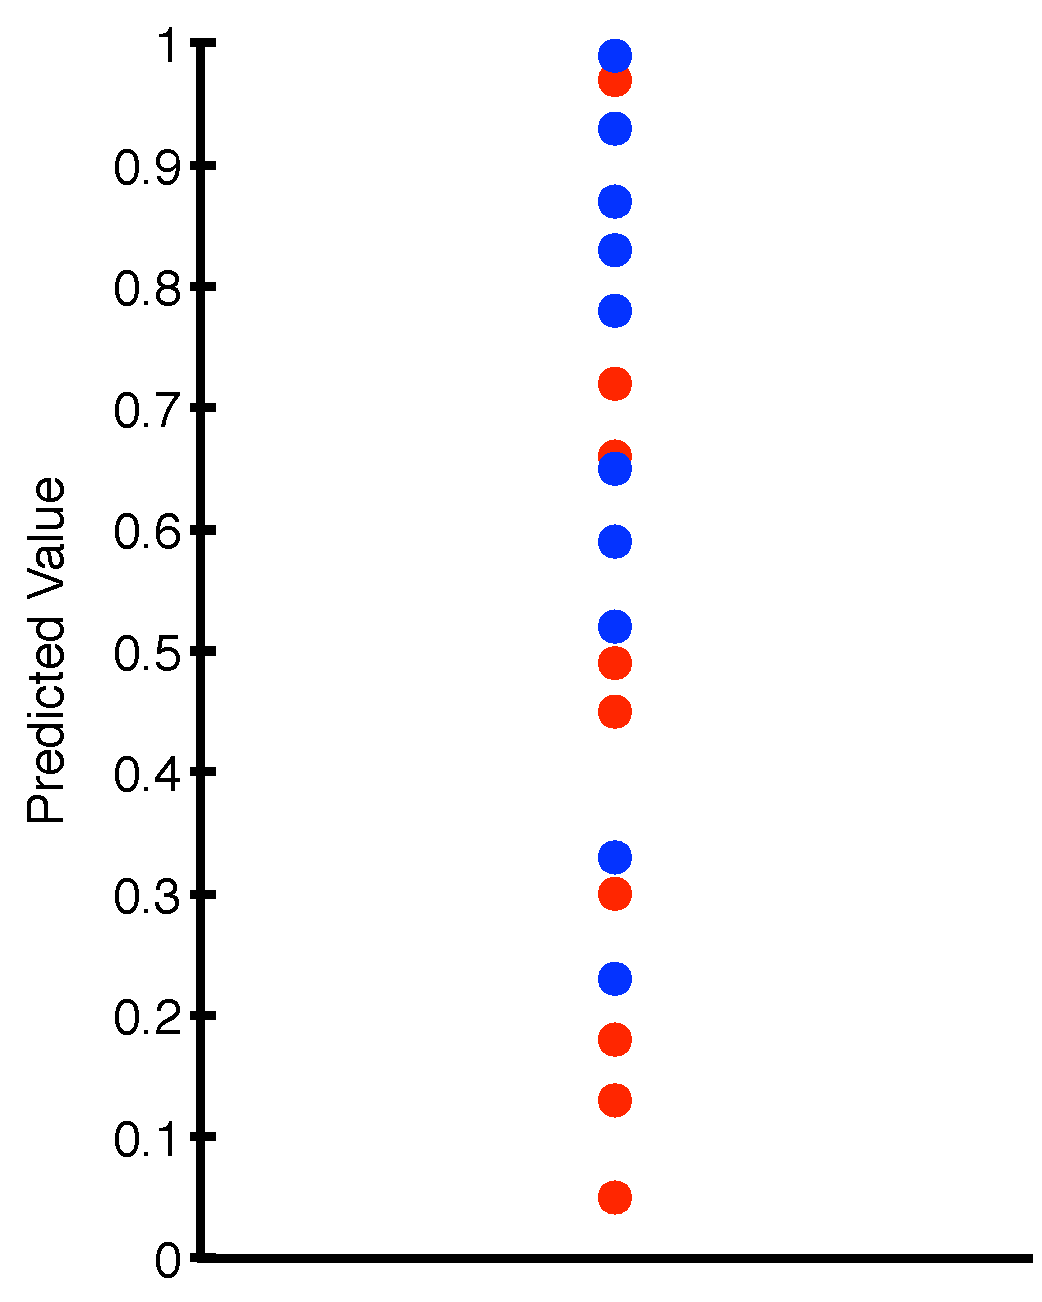
\includegraphics[width=1\textwidth]{lectSup/AUCEx1.pdf} 
\end{column}
\begin{column}{0.2\textwidth}
    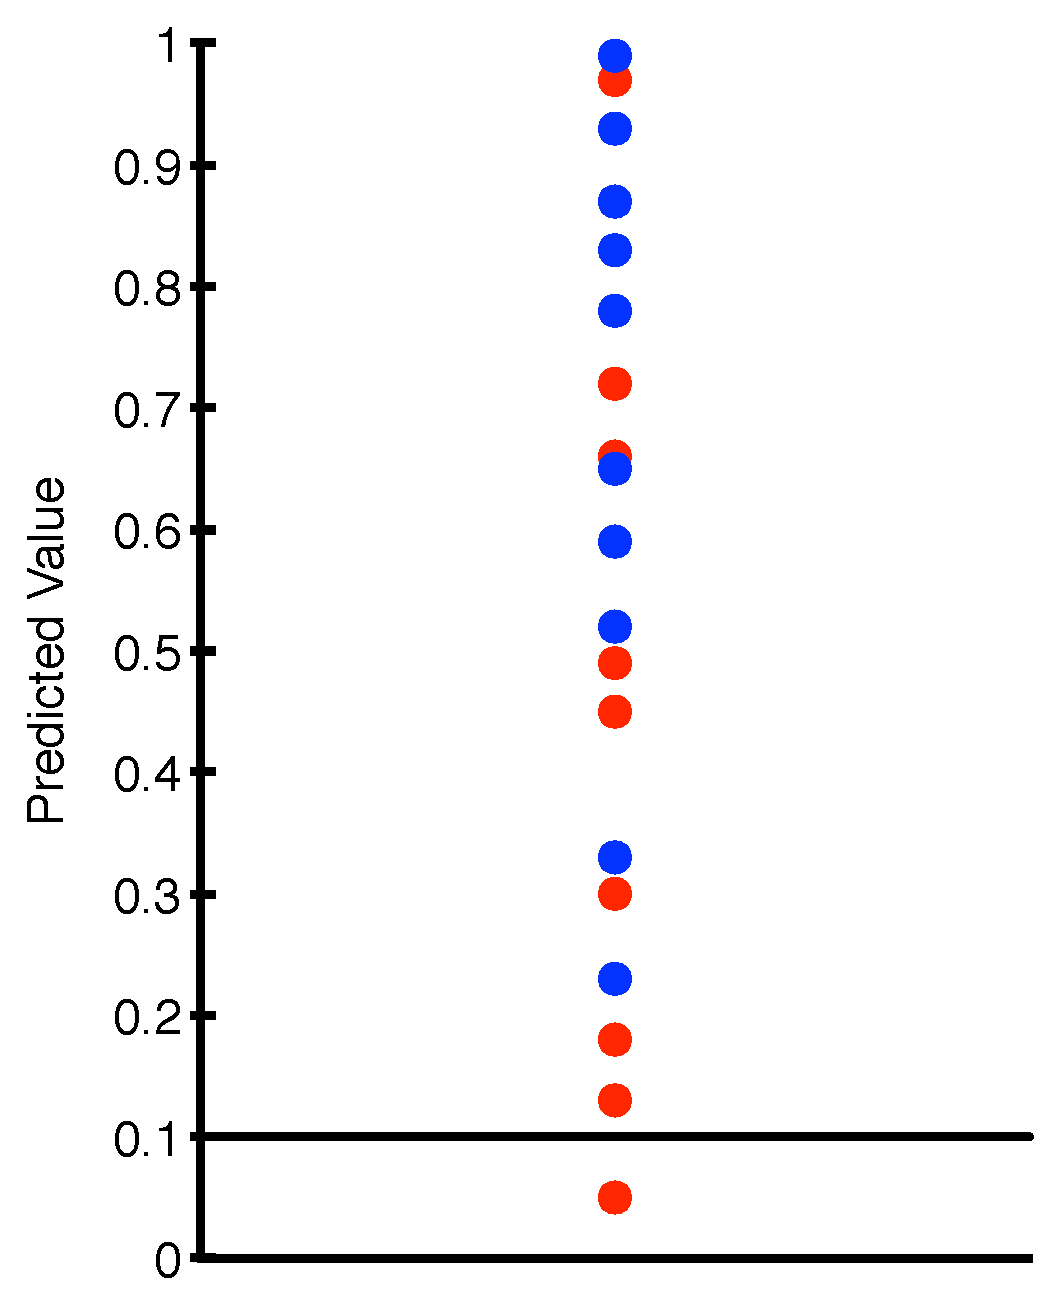
\includegraphics[width=1\textwidth]{lectSup/AUCEx2.pdf} 
\end{column}
\begin{column}{0.2\textwidth}
    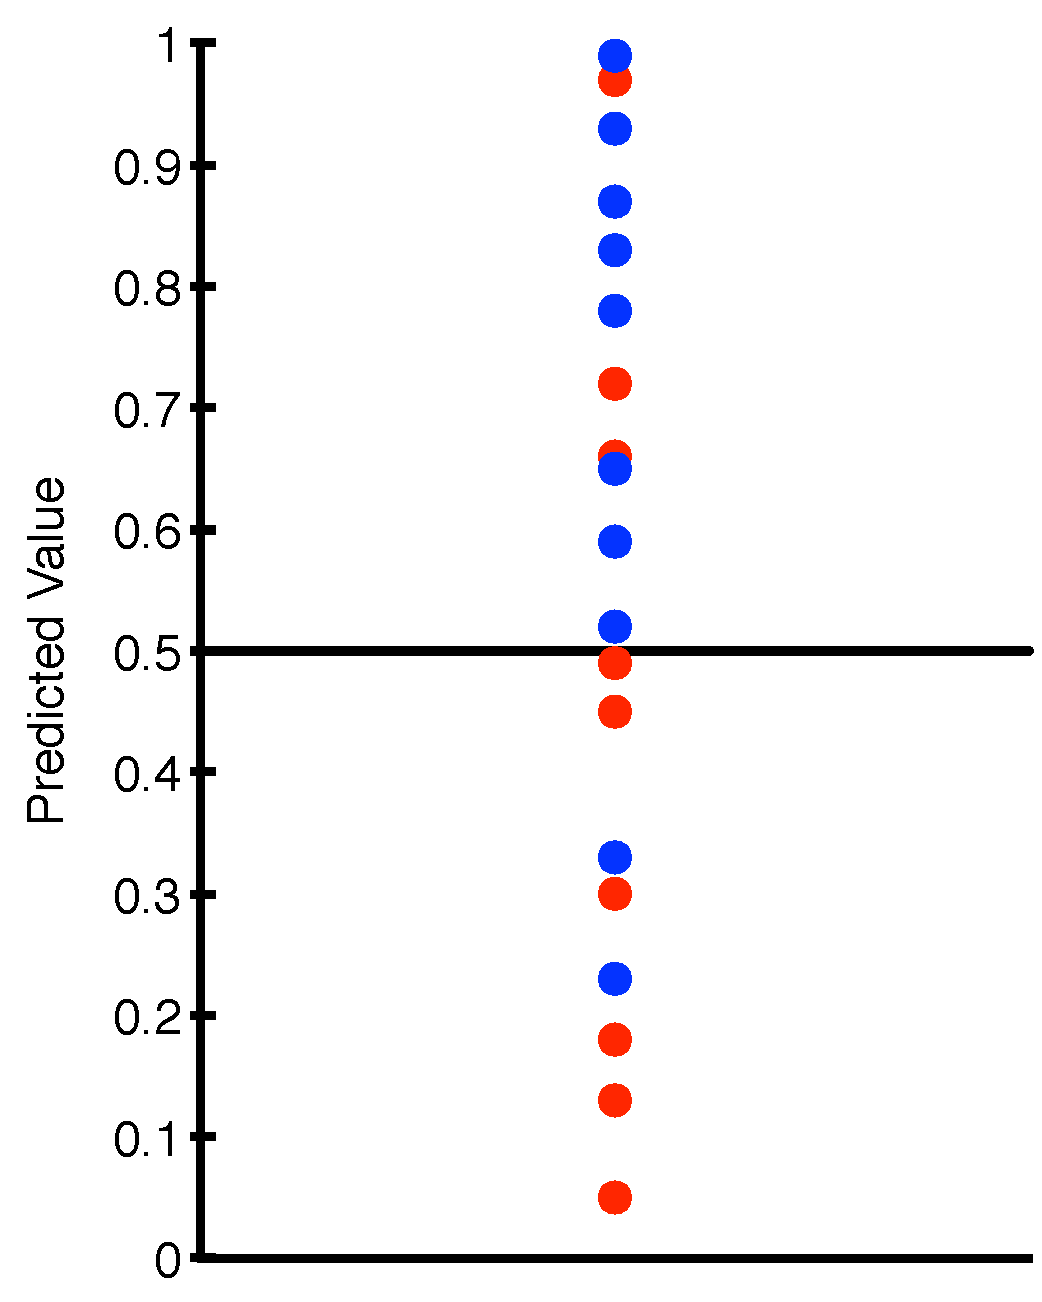
\includegraphics[width=1\textwidth]{lectSup/AUCEx4.pdf} 
\end{column}
\begin{column}{0.2\textwidth}
    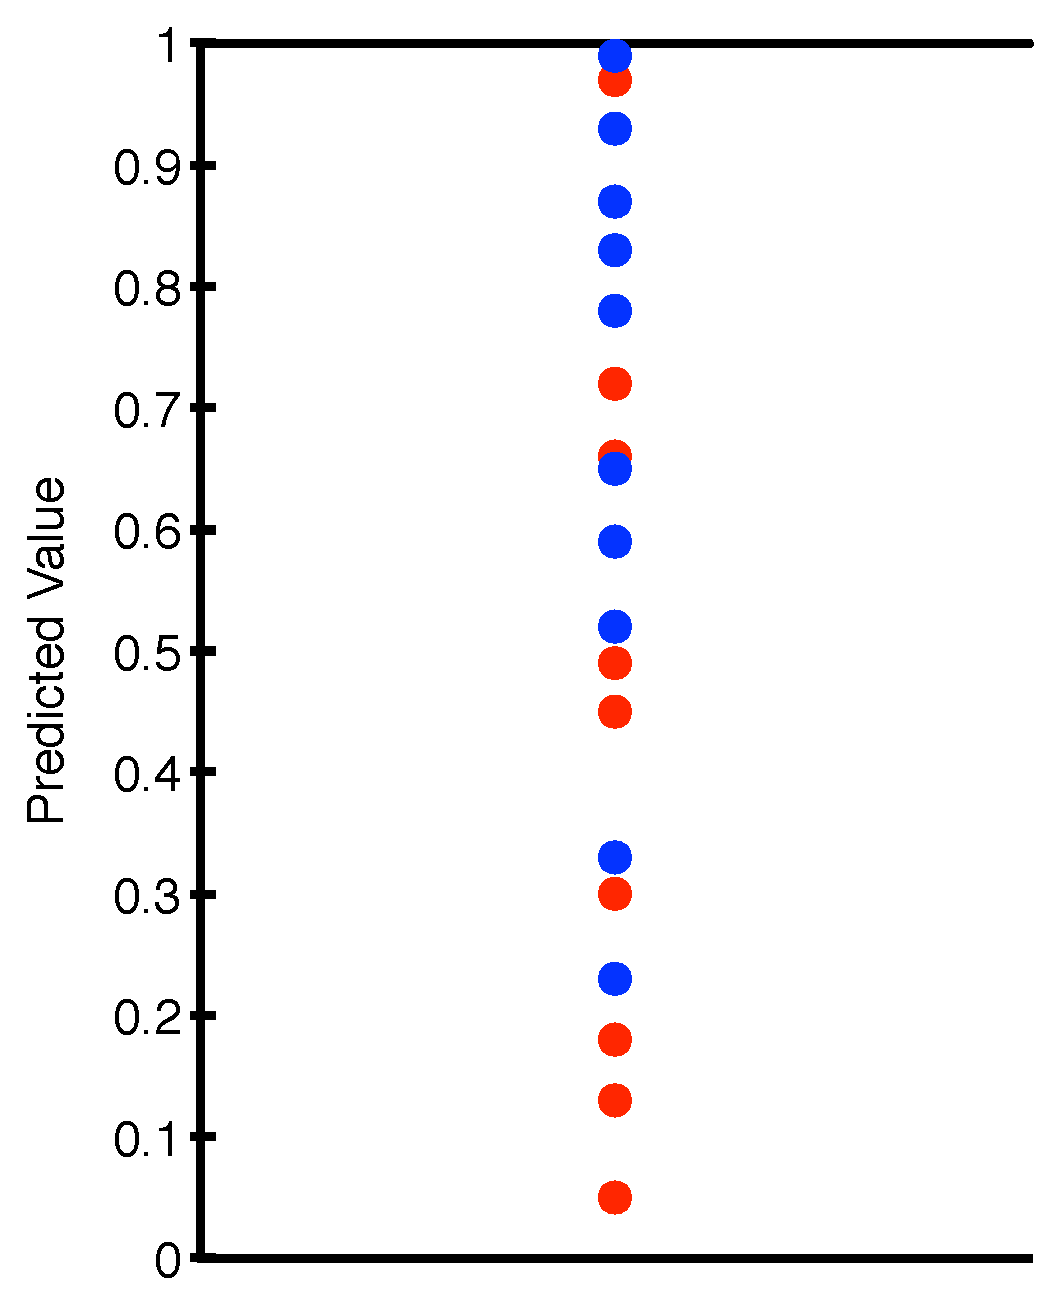
\includegraphics[width=1\textwidth]{lectSup/AUCEx6.pdf} 
\end{column}
\end{columns}
\begin{itemize}
\item Red = Negative cases
\item Blue = Positive cases
\item Start at the bottom (or top)
\item Sweep up (down)
\item Compute the TPR and FPR at each step
\item Plot on ROC
\item Compute AUC
\end{itemize}
\end{frame}
%***********************************************************
%\begin{frame}{Generating the ROC}
%
%\begin{columns}
%\begin{column}{0.5\textwidth}
%    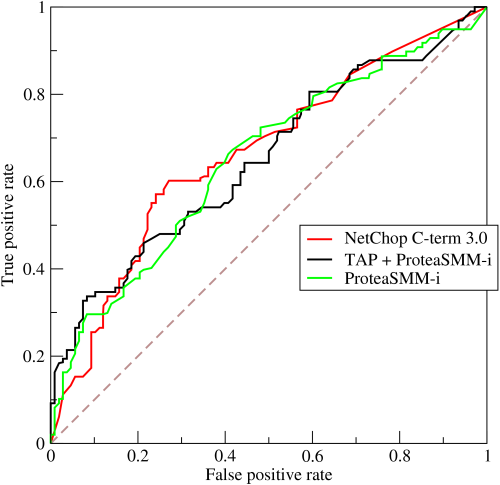
\includegraphics[width=1\textwidth]{lectSup/Roccurves} %https://commons.wikimedia.org/wiki/File:Roccurves.png
%\end{column}
%\begin{column}{0.5\textwidth}
%
%\begin{itemize}
%	\item You set a threshold at one extreme
%	\item Slowly move the threshold 
%	\item Compute the new (FPR, TPR) values
%	\item Plot the pairs
%\end{itemize}
%\end{column}
%\end{columns}
%\end{frame}
%

%***********************************************************
\begin{frame}{Supervised Learning Methodology / Experimental Design}

\begin{itemize}
\item Important to divide available data into 
	\begin{itemize}
	\item Training--used to learn model
	\item Validation--used to see if model useful
	\item Repeat these two, experimenting
	\item Testing--used to evaluate useful models
	\end{itemize}
\item Don't touch testing until ready to eval
	\begin{itemize}
	\item Evaluation on testing must be very last step!
	\item[?] Why?
	\end{itemize}
\end{itemize}
\end{frame}
%***********************************************************
\begin{frame}{Why Test Only Once?}

\begin{columns}
\begin{column}{0.6\textwidth}
\begin{itemize}
\item Overfitting
	\begin{itemize}
	\item It's easy to build a model that exactly fits your data
	\item But doesn't work on new data
	\item Maybe the world has changed 
	\begin{itemize}
	\item Can't do much about this
\end{itemize}
	\item Overfitting  
	\begin{itemize}
	\item You don't want to engineer something that only works on your test data
\end{itemize}
	\end{itemize}
\end{itemize}
 \end{column}
\begin{column}{0.4\textwidth}
    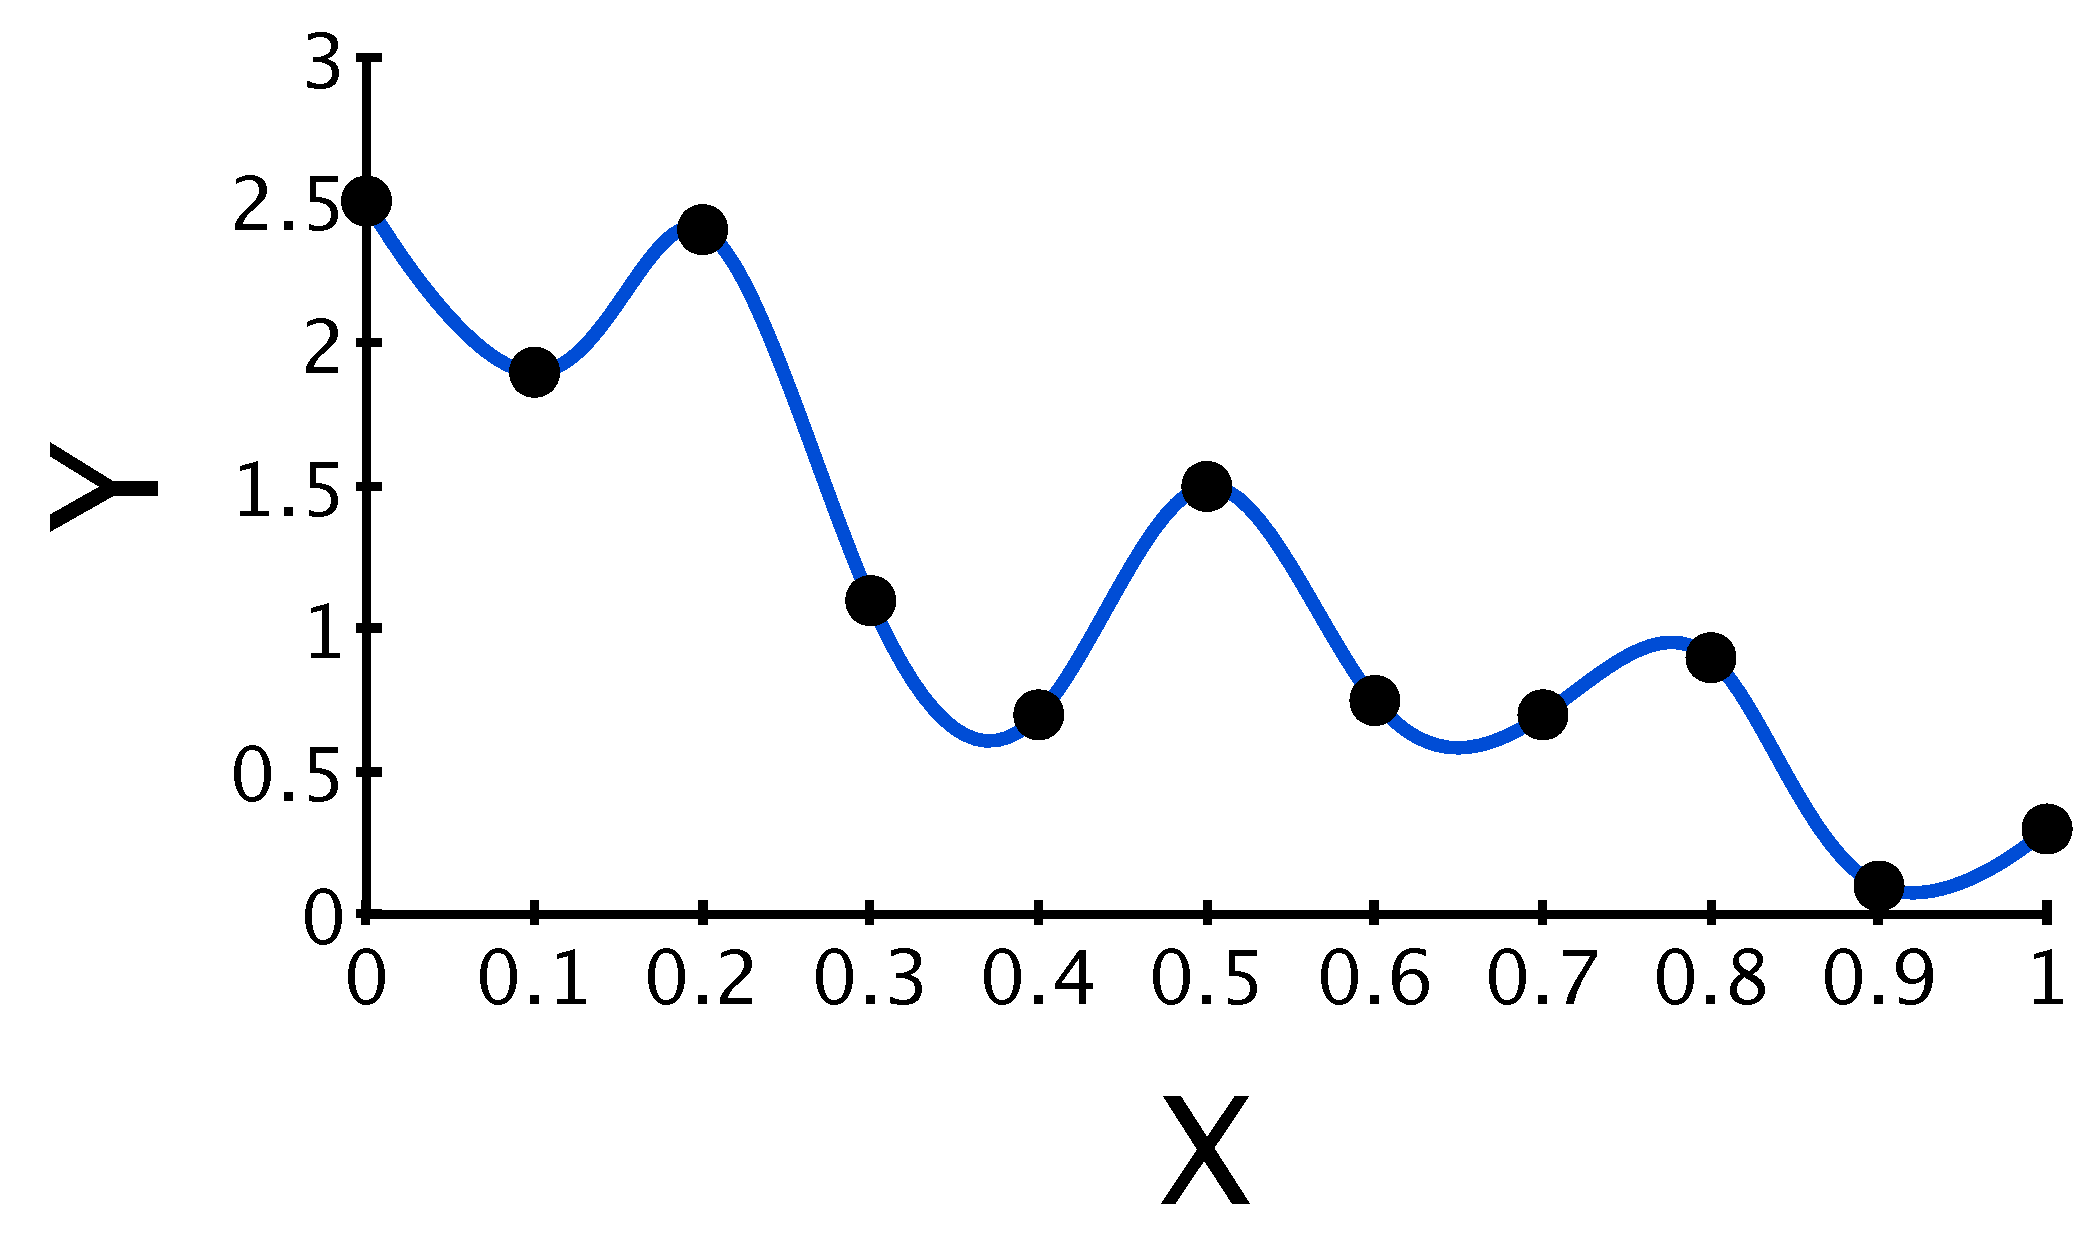
\includegraphics[width=1\textwidth]{lectSup/overfitEx3.pdf} %https://commons.wikimedia.org/wiki/File:Roccurves.png

 \end{column}
 \end{columns}

\end{frame}
%***********************************************************
\begin{frame}[fragile]{How To Perform Testing}

\begin{itemize}
\item One-off
	\begin{itemize}
	\item Divide data into Training, Validation, Testing
	\item Apply validated model(s), get results
	\item[?] What if you don't have a lot of data?
%	\item[?] Problems?
	\end{itemize}
	\end{itemize}

\end{frame}
%***********************************************************
\begin{frame}[fragile]{How To Perform Testing}

\begin{itemize}
\item One-off
	\begin{itemize}
	\item Divide data into Training, Validation, Testing
	\item Apply validated model(s), get results
	\item What if you don't have a lot of data?
	\begin{itemize}
		\item You need to ``reuse'' you data
	\end{itemize}
	\end{itemize}
	\end{itemize}

\end{frame}
%***********************************************************
%\begin{frame}[fragile]{How To Perform Testing}
%
%\begin{itemize}
%\item One-off
%	\begin{itemize}
%	\item Apply validated model(s), get results
%	\item Problems?
%	\item You're done
%	\item You've used up your test set
%	\end{itemize}
%	\end{itemize}
%
%\end{frame}
%***********************************************************
\begin{frame}[fragile]{$k$-Fold Cross-Validation}

	\begin{itemize}
	\item Break data into $k$ random subsets (``folds'')
\begin{SQL}
For i = 1 to $k$ do:
  Train on all folds except i;
  Evaluate learned model on fold i;
Report average results;
\end{SQL}

\item Benefits
	\begin{itemize}
	\item Works for small test sets
	\item $k$ can be large
	\item 10 is commonly used
	\item Needed when the data set is not very large
	\item and / or when there are many parameters
	\end{itemize}
	\end{itemize}
	
% out of scope: Power functions that tell you if you have enough data for your results to be meaningful

\end{frame}
%***********************************************************
\begin{frame}[fragile]{Other techniques for Generating Test Sets}

\begin{itemize}
\item Bootstrap -- random sampling with replacement
\item Jackknife resampling (Leave out one)
\end{itemize}
	

\end{frame}

%***********************************************************
\begin{frame}[fragile]{Bootstrap}

\begin{itemize}
\item Random sampling with replacement
\begin{enumerate}
\item Pick a sample size, $n$
\item Choose $n$ samples from the dataset, WITH replacement
\item Train on the selected samples
\item Test on the non-selected samples in the dataset
\item Average the results
\end{enumerate}
\item Norms
\begin{itemize}
\item $n$ is typically chosen to be the size of the original dataset
\item Repeat the process MANY times (at least 20 or 30, usually hundreds of times)
\item Can also be used to estimate statistics such as a population mean
\end{itemize}
\end{itemize}


\end{frame}
%***********************************************************
\begin{frame}[fragile]{Bootstrap: Pros and Cons}

\begin{itemize}
\item Pros
\begin{itemize}
\item Works well with small datasets
\item Can produce confidence intervals for this approach
\item Non-parametric
\end{itemize}

\item Cons
\begin{itemize}
\item Sample sets are not all the same size
\item Assumes data are independent
\item Not repeatable (samples are different each time)
\end{itemize}
\end{itemize}


\end{frame}
%***********************************************************
\begin{frame}[fragile]{Jackknife}

\begin{itemize}
\item Also know as Leave-one-out 
\item Sampling WITHOUT replacement
\item Older method
%\item Typically used for estimating bias and variance of a statistic
\begin{enumerate}
\item Pick a one sample
\item Train on the remaining samples
\item Test on the selected sample in the dataset
\item Repeat for each sample
\item Average the results
\end{enumerate}
\item Norms
\begin{itemize}
\item Can also be used to estimate statistics such as a population mean
\end{itemize}
\end{itemize}
	

\end{frame}
%***********************************************************
\begin{frame}[fragile]{Jackknife: Pros and Cons}

\begin{itemize}
\item Pros
\begin{itemize}
\item Works well with small datasets
\item Can produce confidence intervals for this approach
\item Non-parametric
\item Uses less computing resources
\end{itemize}

\item Cons
\begin{itemize}
\item Repeatable
\item Assumes data are independent
\end{itemize}
\end{itemize}


\end{frame}
%***********************************************************
\begin{frame}[fragile]{How to Split Data?}

\begin{itemize}
\item Random
\item By time
\item Representative of the data (think about Rice's College system)
\end{itemize}


\end{frame}
%***********************************************************
\begin{frame}[fragile]{Classification or Regression?}

\begin{itemize}
\item Regression
\item ``Real'' value (may be integral)
\item Classification
\item 1 of a limited number of classes
\item[?] How can we convert a regression problem to a classification problem?
\item e.g. Familiarity of a song
% use a threshold
\item[?] How can we make restrict a classification problem to a binary classification problem?
\item E.g. How can we predict if someone is going to get an A, B, or C in this class into a binary classification problem?
% Class A vs Not class A
\end{itemize}


\end{frame}

%***********************************************************
\begin{frame}[fragile]{Rare Class Problems}

\begin{itemize}
\item Problem
  \begin{itemize}
\item Not enough examples to learn how to classify the rare class
\end{itemize}
\item Approaches 
 \begin{itemize}
 \item Oversample the rare class (SMOTE)
 \item Undersample the common class
 \item Create new rare cases based on the minority class
\end{itemize}

\end{itemize}


\end{frame}

%***********************************************************
\begin{frame}[fragile]{Data Preparation}

\begin{itemize}
\item Compute values using the Training set ONLY
\item Apply the EXACT same  transformation to the VALIDATION and TEST sets
\end{itemize}
\end{frame}
%***********************************************************
\begin{frame}[fragile]{Types of Data Preparation / Feature Engineering}

\begin{itemize}
\item Mean normalization - mean 0
$$x' = \frac{x - \textrm{average}(x)}{\textrm{max}(x) - \textrm{min}(x)}$$
\item Standardization - mean 0, std dev = 1
$$ x' = \frac{x -\bar{x}}{\sigma}$$
\item Scaling - min -1, max 1
$$x' = \frac{x - \textrm{min}(x)}{\textrm{max}(x) - \textrm{min}(x)}$$
\item Scale feature vector to unit length across the features
$$x' = \frac{x}{||x||}$$
\end{itemize}
\end{frame}
%***********************************************************
\begin{frame}{Measuring Regression Accuracy}

\begin{itemize}
\item View the list of prediction errors as a vector
\item Can have many loss functions, corresponding to norms
\item Given a vector of errors $\langle \epsilon_1, \epsilon_2, ..., \epsilon_n \rangle$,
$l_p$ norm defined as:
$$\left(\sum_{i = 1}^n |\epsilon_i|^p \right)^{1/p}$$
\item Common loss functions correspond to various norms:
\begin{itemize}
        \item $l_1$ corresponds to mean absolute error
        \item $l_2$ to mean squared error/least squares
\begin{itemize}
\item Most commonly used
\item Convex
\item Easy to compute
\end{itemize}
        \item $l_{\infty}$ corresponds to minimax
\end{itemize}
\end{itemize}
\end{frame}
%***********************************************************
\begin{frame}{Feature Selection}

\begin{itemize}
\item Lots of focus in supervised learning on models
	\begin{itemize}
	\item Linear regression, SVM, kNN, etc.
	\end{itemize}
\item Almost always \textbf{less} important than feature engineering
	\begin{itemize}
	\item That is, most simple models accept $x_i = \langle x_{i,1}, x_{i,2}, ..., x_{i,m} \rangle$	
	\item Do not accept your raw data!
	\item How you ``vectorize'' is often the most important question!
	\end{itemize}
\item Let's consider feature engineering thru an example...
\end{itemize}
\end{frame}
%***********************************************************
\begin{frame}{Web Page Link Feature Selection}

\begin{itemize}
\item Web page link
\begin{itemize}
	\item Location
	\item Font 
	\item Size
	\item Color
	\item $\ldots$
\end{itemize}
\item vs. Deep learning
\begin{itemize}
	\item Use the raw data
	\item E.g. Take a screen shot of the web page
	\item Skip the feature engineering phase
\end{itemize}
\end{itemize}
% this makes a case for Deep Learning, where you use the raw data instead
\end{frame}
%***********************************************************
\begin{frame}{Feature Selection Email}

\centering
    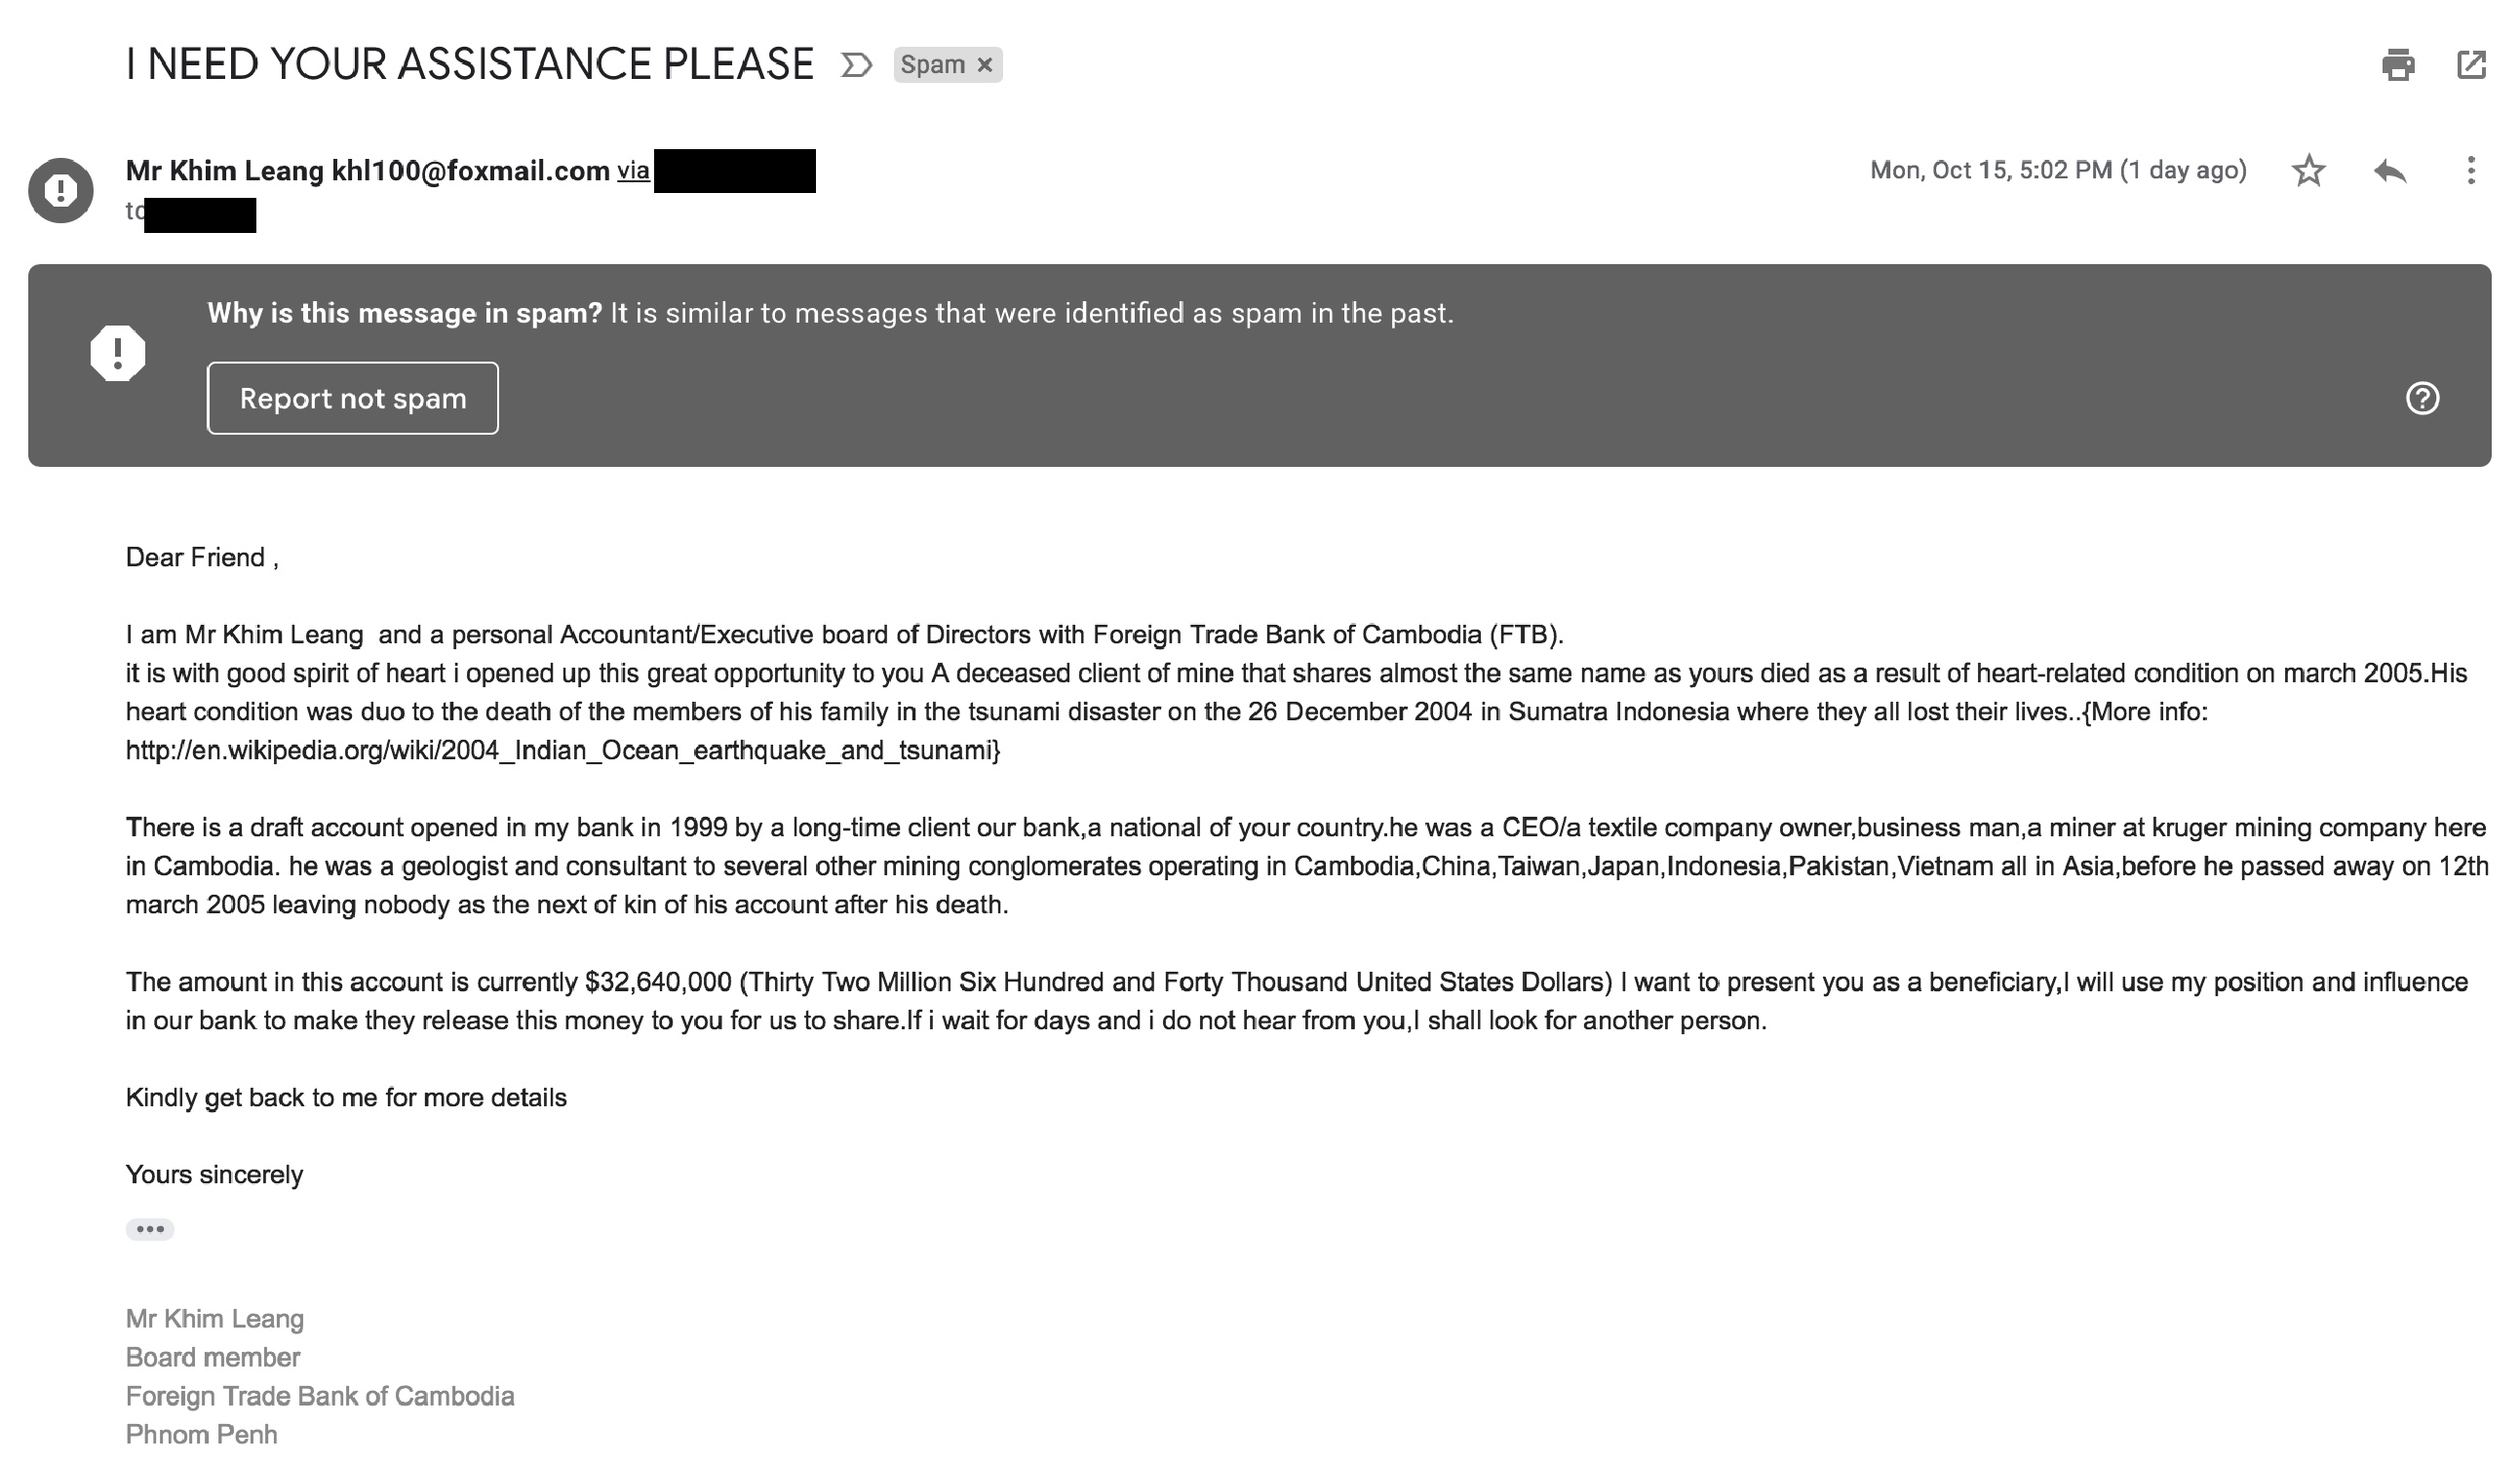
\includegraphics[width=0.9\textwidth]{lectSup/spam.pdf}
\end{frame}
%***********************************************************
\begin{frame}{``Bag of Words''}

\begin{itemize}
\item Might build a dictionary
	\begin{itemize}
	\item That is, map from each of $m$ unique words in corpus
	\item To a number from $\{1...m\}$
	\item Then, each email is a vector $\langle 1, 0, 2, 1, 0, 0, ... \rangle$
	\item $j$th entry is num occurrences of word $j$
	\item Latent Dirichlet Allocation (LDA) uses this approach
	\end{itemize}
\end{itemize}
\end{frame}
%***********************************************************
\begin{frame}{LDA - Latent Dirichlet Allocation}

\begin{columns}
\begin{column}{0.5\textwidth}
\begin{itemize}
\item Recall Lab  - Numpy Arrays % Lab 3
\item LDA - Topic modeling
	\begin{itemize}
	\item Each document in a collection is represented as a mixture of topics
	\item Each topic is represented as a mixture of words.
	\end{itemize}
\end{itemize}
\end{column}
\begin{column}{0.5\textwidth}
    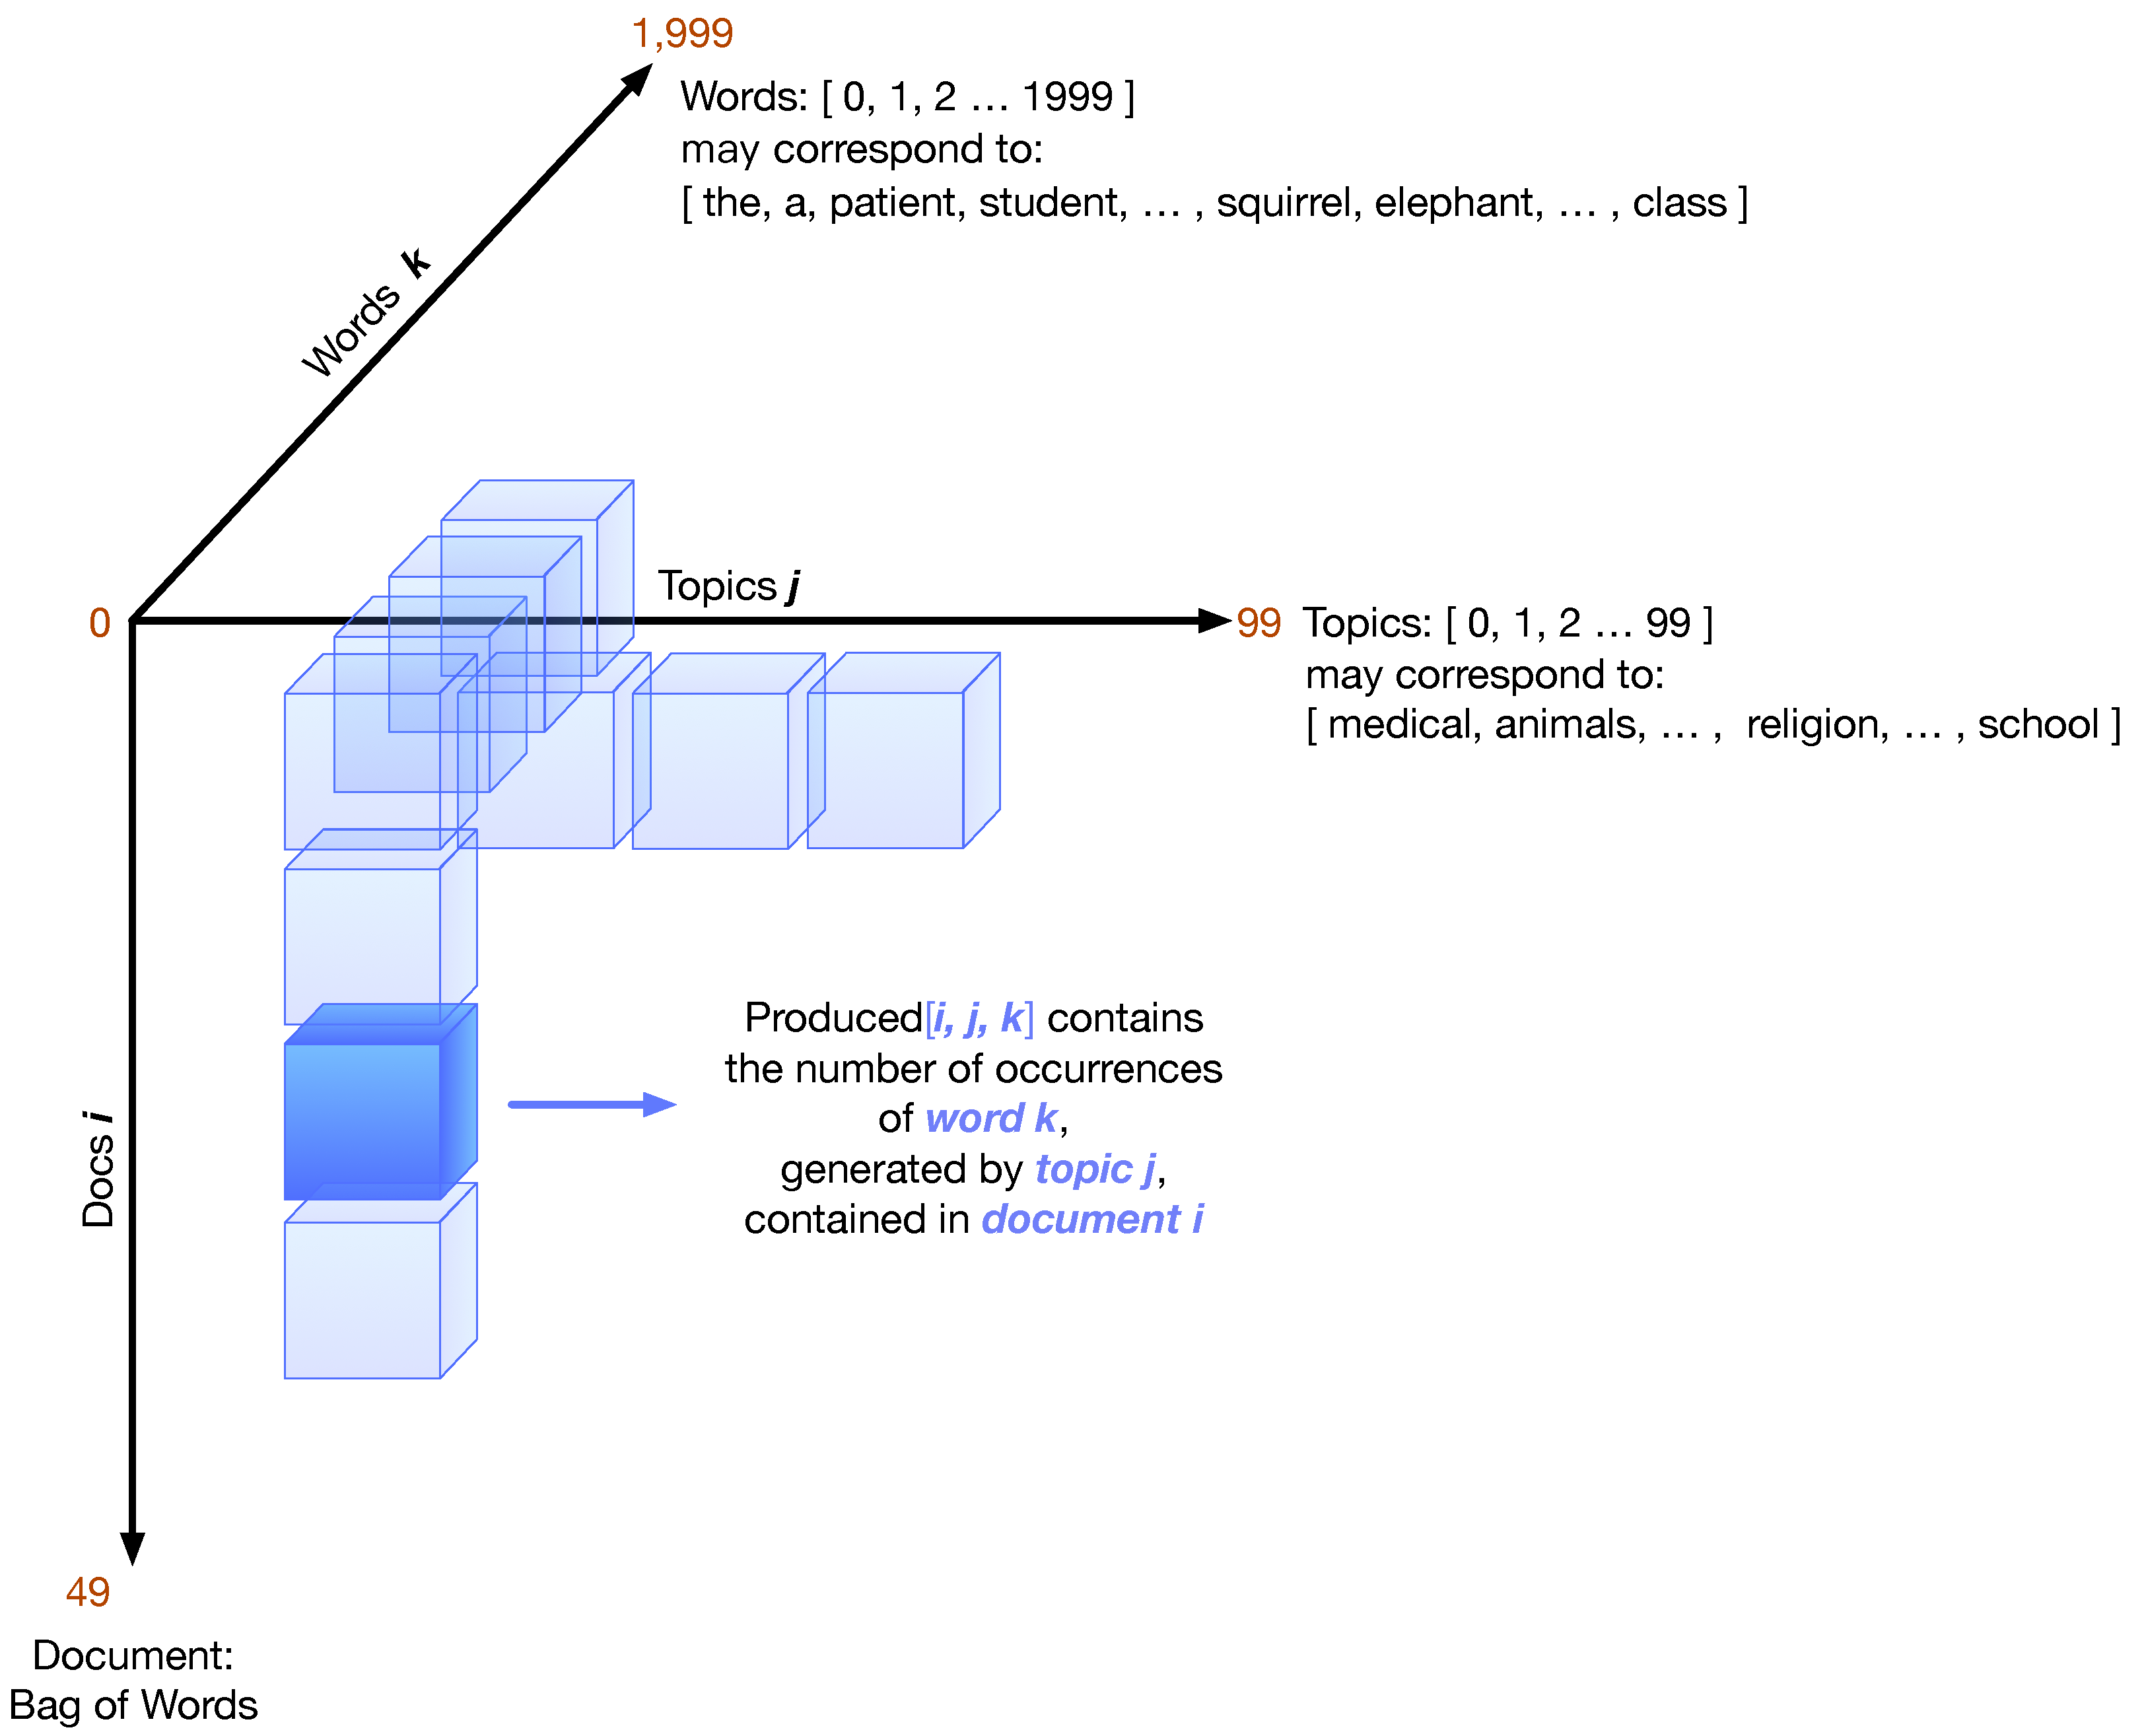
\includegraphics[width=0.9\textwidth]{lectSup/3D.pdf}
\end{column}
\end{columns}

\end{frame}
%***********************************************************
\begin{frame}{``Bag of Words''}

\begin{itemize}
\item Might build a dictionary
	\begin{itemize}
	\item That is, map from each of $m$ unique words in corpus
	\item To a number from $\{1...m\}$
	\item Then, each email is a vector $\langle 1, 0, 2, 1, 0, 0, ... \rangle$
	\item $j$th entry is num occurrences of word $j$
	\item Latent Dirichlet Allocation (LDA) uses this approach
	\item[?] Are there issues with this approach?
	\end{itemize}
\end{itemize}
\end{frame}
%***********************************************************
\begin{frame}{``Bag of Words Issues''}

\begin{enumerate}
\item Sequence information is lost
\begin{itemize}
\item Perhaps it's important to know which words appear early on
\item ... or at the end
\end{itemize}
\item Word importance is lost
\item Some words are equivalent, but look different
\end{enumerate}
\end{frame}
%***********************************************************
\begin{frame}{1. Preserving Sequence Information}

\begin{itemize}
\item Use N-grams
\item N consecutive items
\item \textit{The cow jumped over the moon}
\item[?] What are the 2-grams in this sentence?
\item[?] What are the 3-grams in this sentence?
\end{itemize}
\end{frame}
%***********************************************************
\begin{frame}{N-Grams for Spam Detection}

\begin{itemize}
\item Words in an email might not be suspicious
\item Might be how they are put together
	\begin{itemize}
	\item ``great sorrow''
	\item ``heavy tears''
	\item ``financial institution''
	\end{itemize}
\item Idea: also include all 2-grams, 3-grams, 4-grams, etc. as features
\end{itemize}
\end{frame}
%***********************************************************
\begin{frame}{N-gram Example}

\begin{itemize}
\item \textit{The cow jumped over the moon}
\end{itemize}
\begin{columns}[t]
\begin{column}{0.5\textwidth}
\begin{itemize}
\item 2-grams / bigrams
\begin{enumerate}
\item \textit{The cow}
\item \textit{cow jumped}
\item  \textit{jumped over}
\item \textit{over the}
\item \textit{the moon}
\end{enumerate}
\end{itemize}
\end{column}
\begin{column}{0.5\textwidth}
\begin{itemize}
\item 3-grams / trigrams
\begin{enumerate}
\item  \textit{The cow jumped}
\item \textit{cow jumped over}
\item \textit{jumped over the}
\item \textit{over the moon}
\end{enumerate}
\end{itemize}
\end{column}
\end{columns}
\begin{itemize}
\item[?] Issues with N-grams?
\end{itemize}
\end{frame}
%***********************************************************
\begin{frame}{Issues with N-grams}

\begin{columns}
\begin{column}{0.5\textwidth}
\begin{itemize}
\item \# of combinations explodes
\item The data dimensionality can get to billions
\item But the feature vector is typically sparse
\item Again, recall the numpy array lab - many entries in the matrix were zero
\end{itemize}
\end{column}
\begin{column}{0.5\textwidth}
    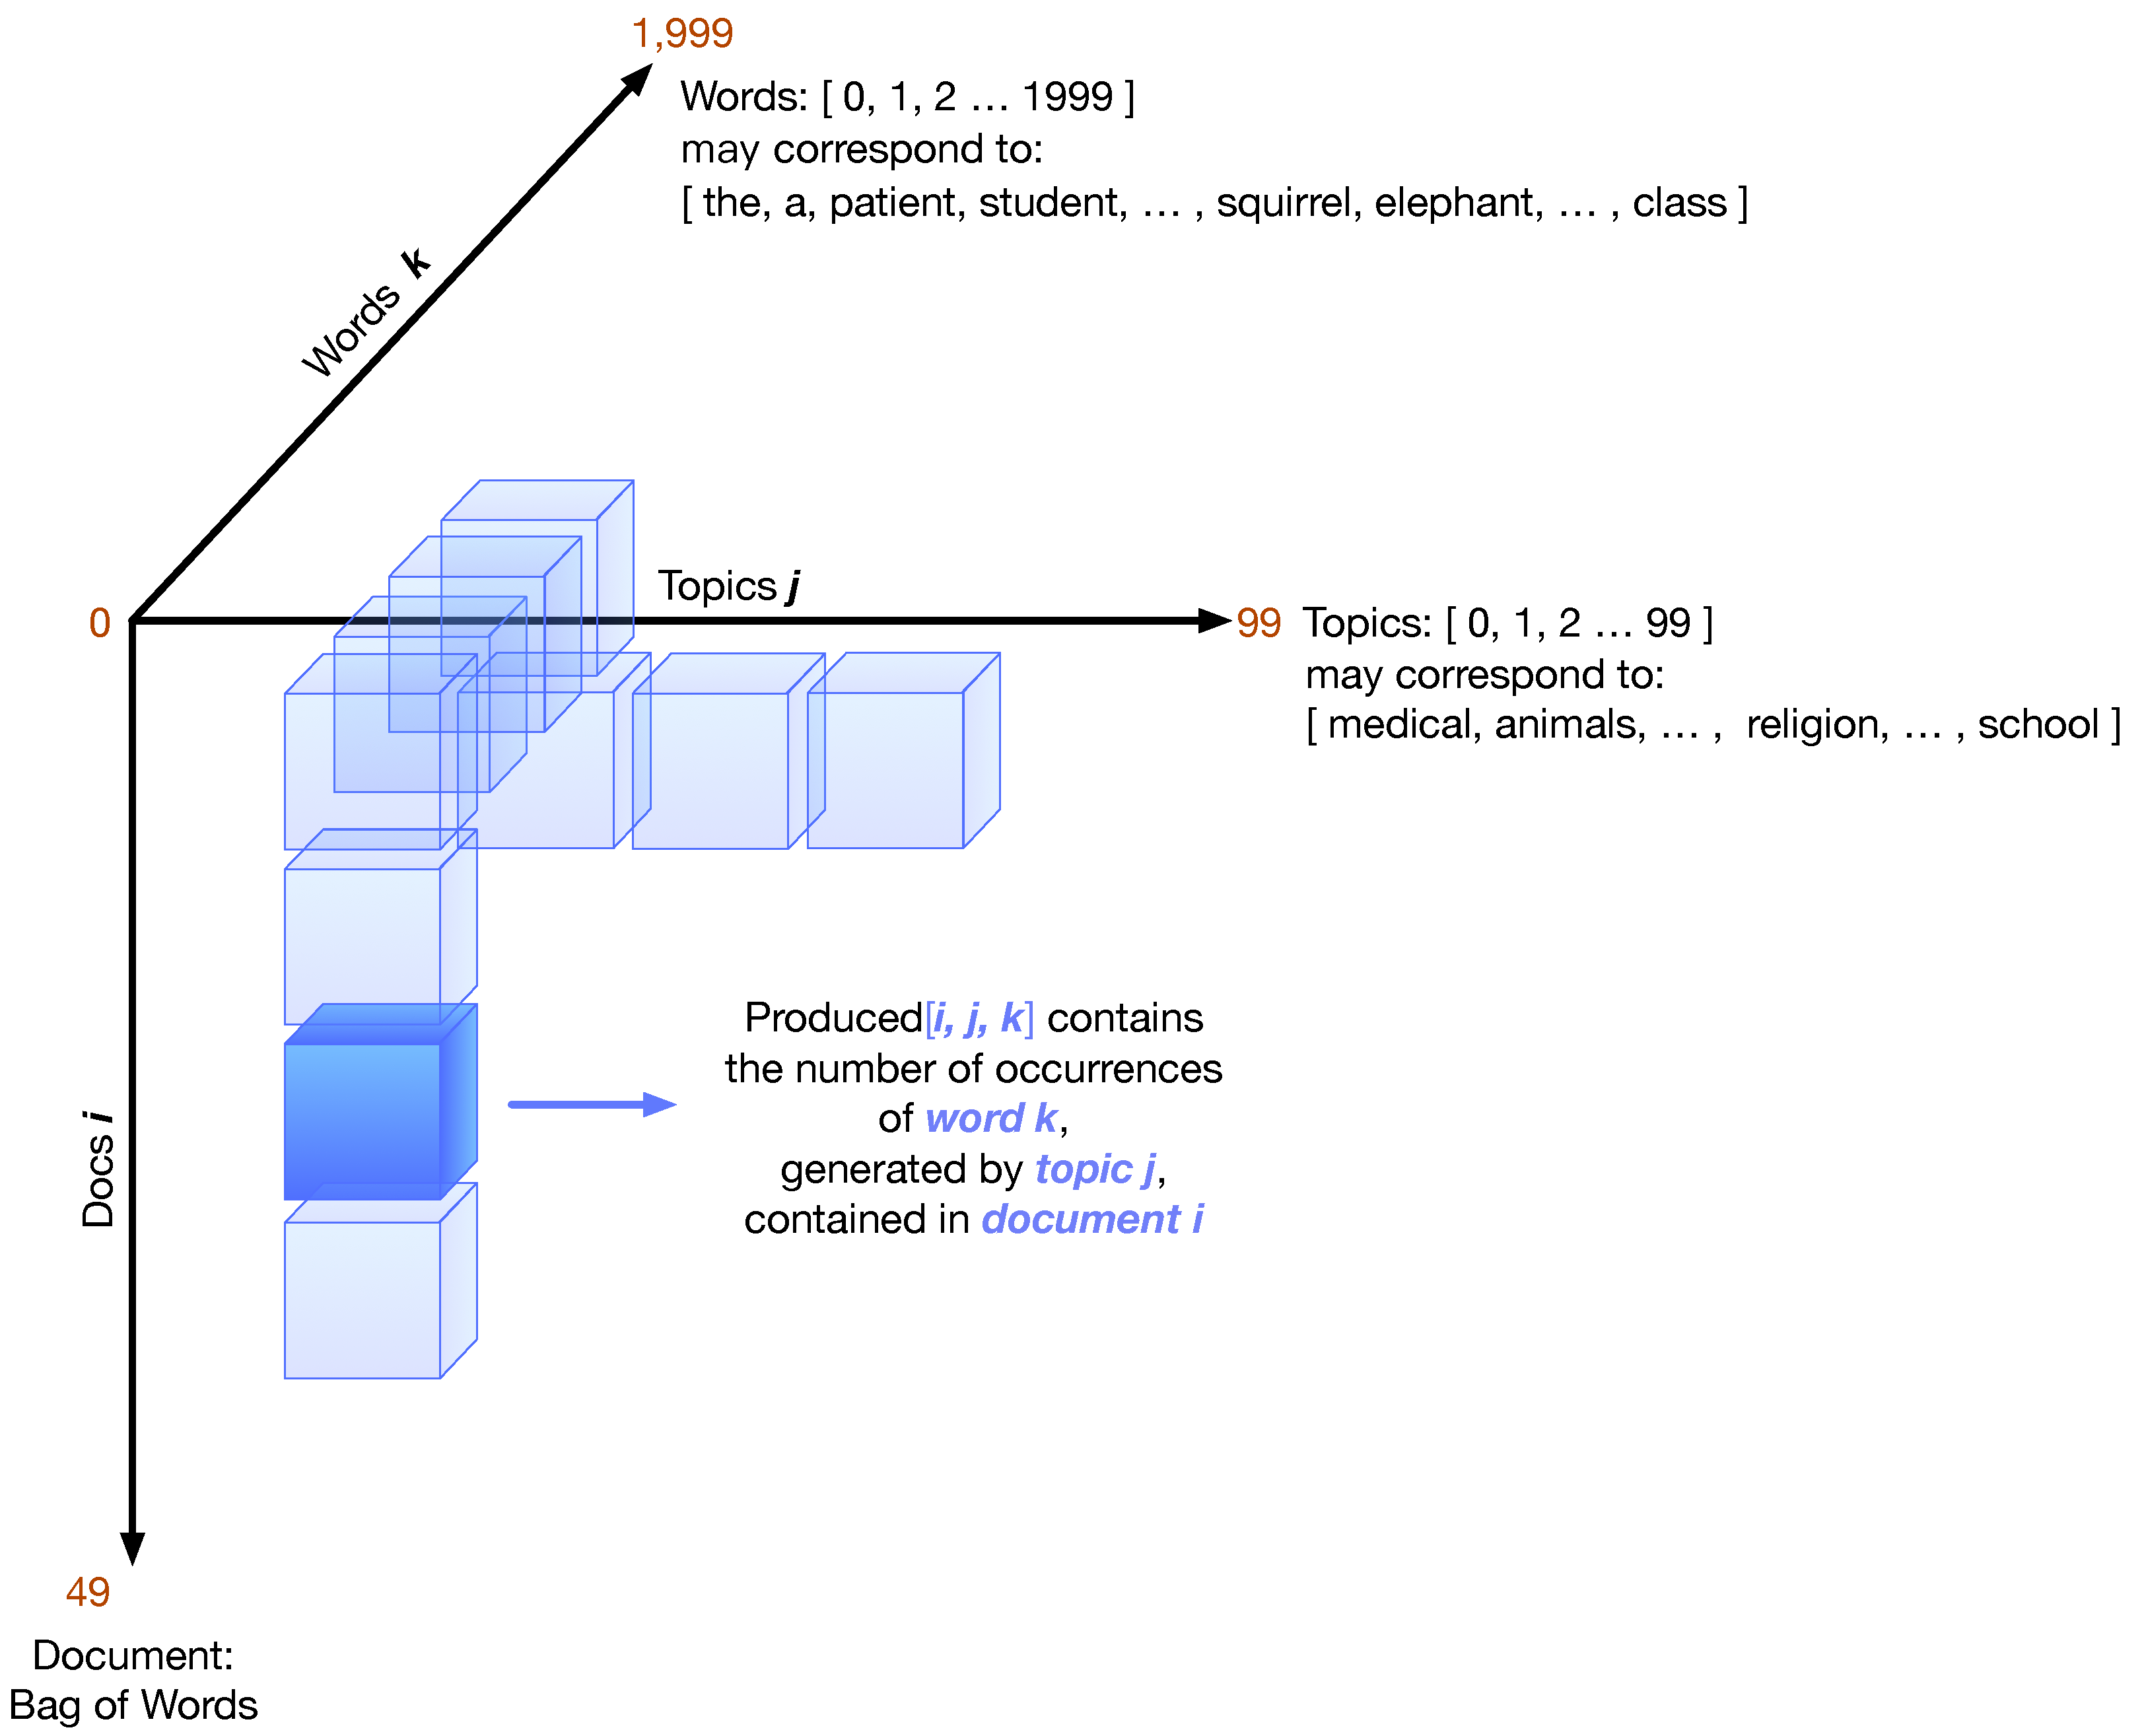
\includegraphics[width=0.9\textwidth]{lectSup/3D.pdf}
\end{column}
\end{columns}
\end{frame}
%***********************************************************
\begin{frame}{``Bag of Words Issues''}

\begin{enumerate}
\item \textcolor{lightgray}{ Sequence information is lost}
\item Word importance is lost
\begin{itemize}
\item Some words are more significant than others
\end{itemize}
\item \textcolor{lightgray}{ Some words are equivalent, but look different}
\end{enumerate}
\end{frame}
%***********************************************************
\begin{frame}{2. Word importance is lost}

\begin{enumerate}
\item Eliminate ``Stop Words''
\begin{itemize}
\item Common words are often filtered out
\item ... a, an, the, is, with ...
\end{itemize}

\item TF-IDF
\end{enumerate}
\end{frame}
%***********************************************************
\begin{frame}{TF-IDF}

\begin{itemize}
\item Term Frequency, Inverse Document Frequency
\item Two components
\begin{enumerate}

\item ``Term Frequency''  --  frequency of each word in the document
	\begin{itemize}
	\item[]
	$$TF = \frac{\textrm{num occurs of word in doc}}{\textrm{num words in doc}}$$
	\end{itemize}
\item ``Inverse Document Frequency'' -- rareness of the word in the corpus
	\begin{itemize}
	\item[] 
	$$IDF = \log \frac{\textrm{num of docs}}{\textrm{num of docs having the word + 1}}$$
	\end{itemize}
\end{enumerate}
\item[?] Why ``+1''? % to avoid division by zero
\item TD-IDF defined as $TF \times IDF$
\end{itemize}
\end{frame}
%***********************************************************
\begin{frame}{TF-IDF Intuition}

\begin{itemize}
\item[]
	$$TF = \frac{\textrm{num occurs of word in doc}}{\textrm{num words in doc}}$$
	$$IDF = \log \frac{\textrm{num of docs}}{\textrm{num of docs having the word + 1}}$$
$$TD-IDF = TF \times IDF$$

\item Words that appear more often have a higher value
\item Longer documents are expected to have more words, so we TF uses the number of words in the document
\item Words that are rare should have a higher value
\end{itemize}
\end{frame}
%***********************************************************
\begin{frame}{``Bag of Words Issues''}

\begin{enumerate}
\item \textcolor{lightgray}{ Sequence information is lost}
\item \textcolor{lightgray}{Word importance is lost}
\item Some words are equivalent, but look different
\begin{itemize}
\item Stemming - reduce a word to its base
\item Remove punctuation? % might or might not choose to do this
\item Ignore capitalization? % might or might not choose to do this
\end{itemize}
\end{enumerate}
\end{frame}
%***********************************************************
\begin{frame}{Other Features for Spam Detection}

\begin{itemize}
\item Country of sender
\item Number of words in email
\item Time of day sent
\item Was the email sent previously? Does it include an email I sent?
\item Recipient list disclosed? If not, indicative of spam
\item Capitalization
\end{itemize}
\end{frame}
%***********************************************************
\begin{frame}{Feature Engineering}

\begin{itemize}
\item Applying \textcolor{red}{domain} knowledge to create useful features
\item Examples
\begin{itemize}
\item Spam email features (previous slide)
\item	Predicting intracranial pressure crises: Time since last crisis
\item ``Binning'' values: Low / Medium / High
\item Time series features
\begin{itemize}
	\item Window
	\item Min / Max / Mean / Median
	\item Variance
	\item Skew / Kurtosis 
\end{itemize}
\end{itemize}

\end{itemize}
    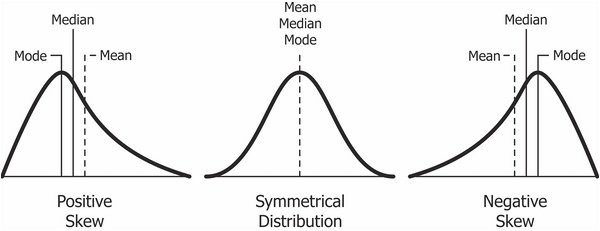
\includegraphics[width=0.5\textwidth]{lectSup/skew.jpeg}
\end{frame}
%***********************************************************
\begin{frame}{Feature Engineering: Don't Cheat!}

\begin{itemize}
\item You can only use the information available at the prediction time
\item Examples
\begin{itemize}
\item Predicting Intracranial pressure crises:  Whether or not the patient died % can't just use epochs from patients who lived / died / had crises / didn't have crises
\end{itemize}

\end{itemize}
\end{frame}
%***********************************************************
\begin{frame}{Feature Engineering: Avoid / Minimize Bias}

\begin{itemize}
\item If our examples of spam all come from certain countries, we are more likely to categorize ANY email from those countries as spam

\end{itemize}
\end{frame}
%***********************************************************
\begin{frame}{Feature Selection}

\begin{itemize}
\item Finding the helpful features
\item[] Why not use them all?
\end{itemize}
\end{frame}
%***********************************************************
\begin{frame}{Feature Selection}

\begin{itemize}
\item Finding the helpful features
\item Why not use them all?
\begin{enumerate}
\item To avoid overfitting
\item To reduce complexity
\item To enable faster training
\item To avoid having a sparse feature space where $n \ll p$ (Curse of dimensionality)
\end{enumerate}
\end{itemize}
\end{frame}
%***********************************************************
\begin{frame}{Techniques for Feature Selection}

\begin{enumerate}
\item Embedded methods
	\begin{enumerate}
	\item LASSO Regularization (last lecture)
	\end{enumerate}
\item Filter methods
	\begin{enumerate}
	\item Statistical measures of relevance (e.g. Chi squared, information gain, correlation coefficient)
	\item Often univariate 
	\end{enumerate}
\item Wrapper methods
	\begin{enumerate}
	\item Search problem
	\item Try different combinations of features
	\item Compare results
	\item Can be Greedy, Stochastic, Exhaustive, Forward, Backward
	% Backward - start with all, remove one by one
	% Forward - add one at a time, while accuracy increases
	\end{enumerate}
\end{enumerate}
\end{frame}

%***********************************************************
\begin{frame}{A4}

\begin{itemize}
\item kNN classifier to classify text documents
\item Most frequent label in the $k$ nearest neighbors
\item Using the $L_2$ norm
\item Implemented in PySpark
\item Data
\begin{itemize}
\item ``20 newsgroups'' data set
\item Old-school blog
\item 19,997 documents
\end{itemize}
\item Labels
\begin{itemize}
\item 20 categories
\item Which newsgroup the document was posted in
\item ... comp.graphics, rec.autos, sci.space, ...
\end{itemize}
\end{itemize}
\end{frame}

%***********************************************************
\begin{frame}{Questions?}
\begin{itemize}
	\item What do we know now that we didn't know before?

	\item How can we use what we learned today?
\end{itemize}
\end{frame}

\end{document}
